\documentclass[10pt,letterpaper]{article}
\usepackage[margin=0.68in]{geometry}
\usepackage[T1]{fontenc}\usepackage{lmodern}
\usepackage{graphicx,xcolor,booktabs,array,longtable,fancyhdr,amsmath,amssymb,pdflscape}
\usepackage[hidelinks]{hyperref}
\definecolor{navy}{HTML}{153047}\definecolor{teal}{HTML}{007C89}
\definecolor{muted}{HTML}{526574}\definecolor{alert}{HTML}{A42D2D}
\setlength{\parindent}{0pt}\setlength{\parskip}{6pt}
\setlength{\headheight}{14pt}\pagestyle{fancy}\fancyhf{}
\fancyhead[L]{\small\color{navy}Hand BASIC preview atlas}
\fancyhead[R]{\small\color{muted}500 MHz to 67 GHz}
\fancyfoot[L]{\footnotesize\color{muted}6 \ensuremath{\mu\mathrm{m}} LTC-25000 / 700 \ensuremath{\mu\mathrm{m}} EME-G730 / as-supplied: no ground plane}
\fancyfoot[R]{\small\thepage}
\newcommand{\pageTitle}[2]{{\LARGE\bfseries\color{navy}#1}\par{\small\color{muted}#2}\par\vspace{7pt}}
\newcommand{\subhead}[1]{\par\addvspace{7pt}\noindent{\large\bfseries\color{teal}#1}\par\nobreak\vspace{2pt}}
\newcommand{\callout}[1]{\begingroup\setlength{\fboxsep}{8pt}\fcolorbox{alert}{white}{\parbox{\dimexpr\linewidth-18pt\relax}{\small\color{alert}#1}}\endgroup\par}
\newcommand{\minihead}[1]{\par\addvspace{4pt}\noindent{\bfseries\color{navy}#1}\par\nobreak\vspace{1pt}}
\newcommand{\response}[2]{\begin{center}\includegraphics[width=.9\linewidth,height=.27\textheight,keepaspectratio]{assets/#1.png}\par\smallskip{\footnotesize\color{muted}#2}\end{center}}
\newcommand{\gdsfig}[2]{\begin{center}\includegraphics[width=.96\linewidth,height=.26\textheight,keepaspectratio]{assets/gds-#1.png}\par\smallskip{\footnotesize\color{muted}#2}\end{center}}
\newcommand{\preview}[2]{\begin{center}\includegraphics[width=.96\linewidth,height=.49\textheight,keepaspectratio]{assets/#1.png}\par\smallskip{\footnotesize\color{muted}#2}\end{center}}
\hypersetup{pdftitle={Hand BASIC Preview Atlas: LTC-25000 and EME-G730},pdfauthor={RF Test Designer},pdfsubject={500 MHz to 67 GHz source previews and model applicability}}
\begin{document}
\pageTitle{Hand BASIC preview atlas}{RF test structures for the supplied copper / polyimide / mold-resin stack}
{\huge\bfseries\color{teal}500 MHz to 67 GHz}\par
\vspace{6pt}
This report collects source-derived previews of all ten Hand BASIC programs in the parent folder: eight RF programs and two mathematical utilities. It records the requested physical stack, preserves the cardinal MPI probe arrangement, and identifies the model changes needed before electrical dimensions or performance can be assigned to this stack.
\subhead{Physical configuration supplied by the user}
\par\noindent\begin{tabular}{@{}p{.37\linewidth}p{.58\linewidth}@{}}\toprule
Frequency range & 0.500 to 67.000 GHz\\
Top copper thickness & 2.2 \ensuremath{\mu\mathrm{m}}\\
Insulation & FUJIFILM LTC-25000 polyimide, 6 \ensuremath{\mu\mathrm{m}} cured thickness\\
Substrate & EME-G730 mold resin, 700 \ensuremath{\mu\mathrm{m}} thick\\
RF grounds, as supplied & Top-side GSG grounds only; no continuous ground plane\\
RF grounds, GDSII cells & Continuous ground plane directly under the 6 \ensuremath{\mu\mathrm{m}} polyimide (layer 1), added by request\\
Installed probes & MPI TITAN, rated to 67 GHz, 150 \ensuremath{\mu\mathrm{m}} adjacent-tip pitch\\\bottomrule
\end{tabular}\par
\vspace{9pt}
\callout{\textbf{The existing grounded models do not predict the supplied stack.} The BASIC programs synthesize microstrip and, in the ring launch, grounded CPW using a homogeneous dielectric and a continuous return plane. That plane is absent in the supplied stack. All printed impedances, widths, electrical lengths, mode frequencies and response curves inherited from those models are hypothetical reference results. They apply to the GDSII unit cells only because those cells add the plane the models assume.}
\subhead{What this delivery establishes}
The atlas supplies native-source artwork, port assignments, drawing-command records and reproducible generation files. It includes 14 RF drawing views and two utility text views. Schematics show program concepts and are not scaled mask layouts. The mobile Hand BASIC app was not executed.
Published material information located for LTC-25000 and EME-G730 did not establish complex permittivity over this frequency range. No actual-stack impedance, loss, crosstalk, leakage isolation or ring resonance is asserted in this report.
\vfill
{\small\color{muted}Drawing revision 3 November 2026. PDF typeset with pdfLaTeX. Legacy numerical equations remain unchanged.}
\newpage
\pageTitle{Stack and RF return path}{The insulation thickness is not the full electromagnetic substrate height}
\begin{center}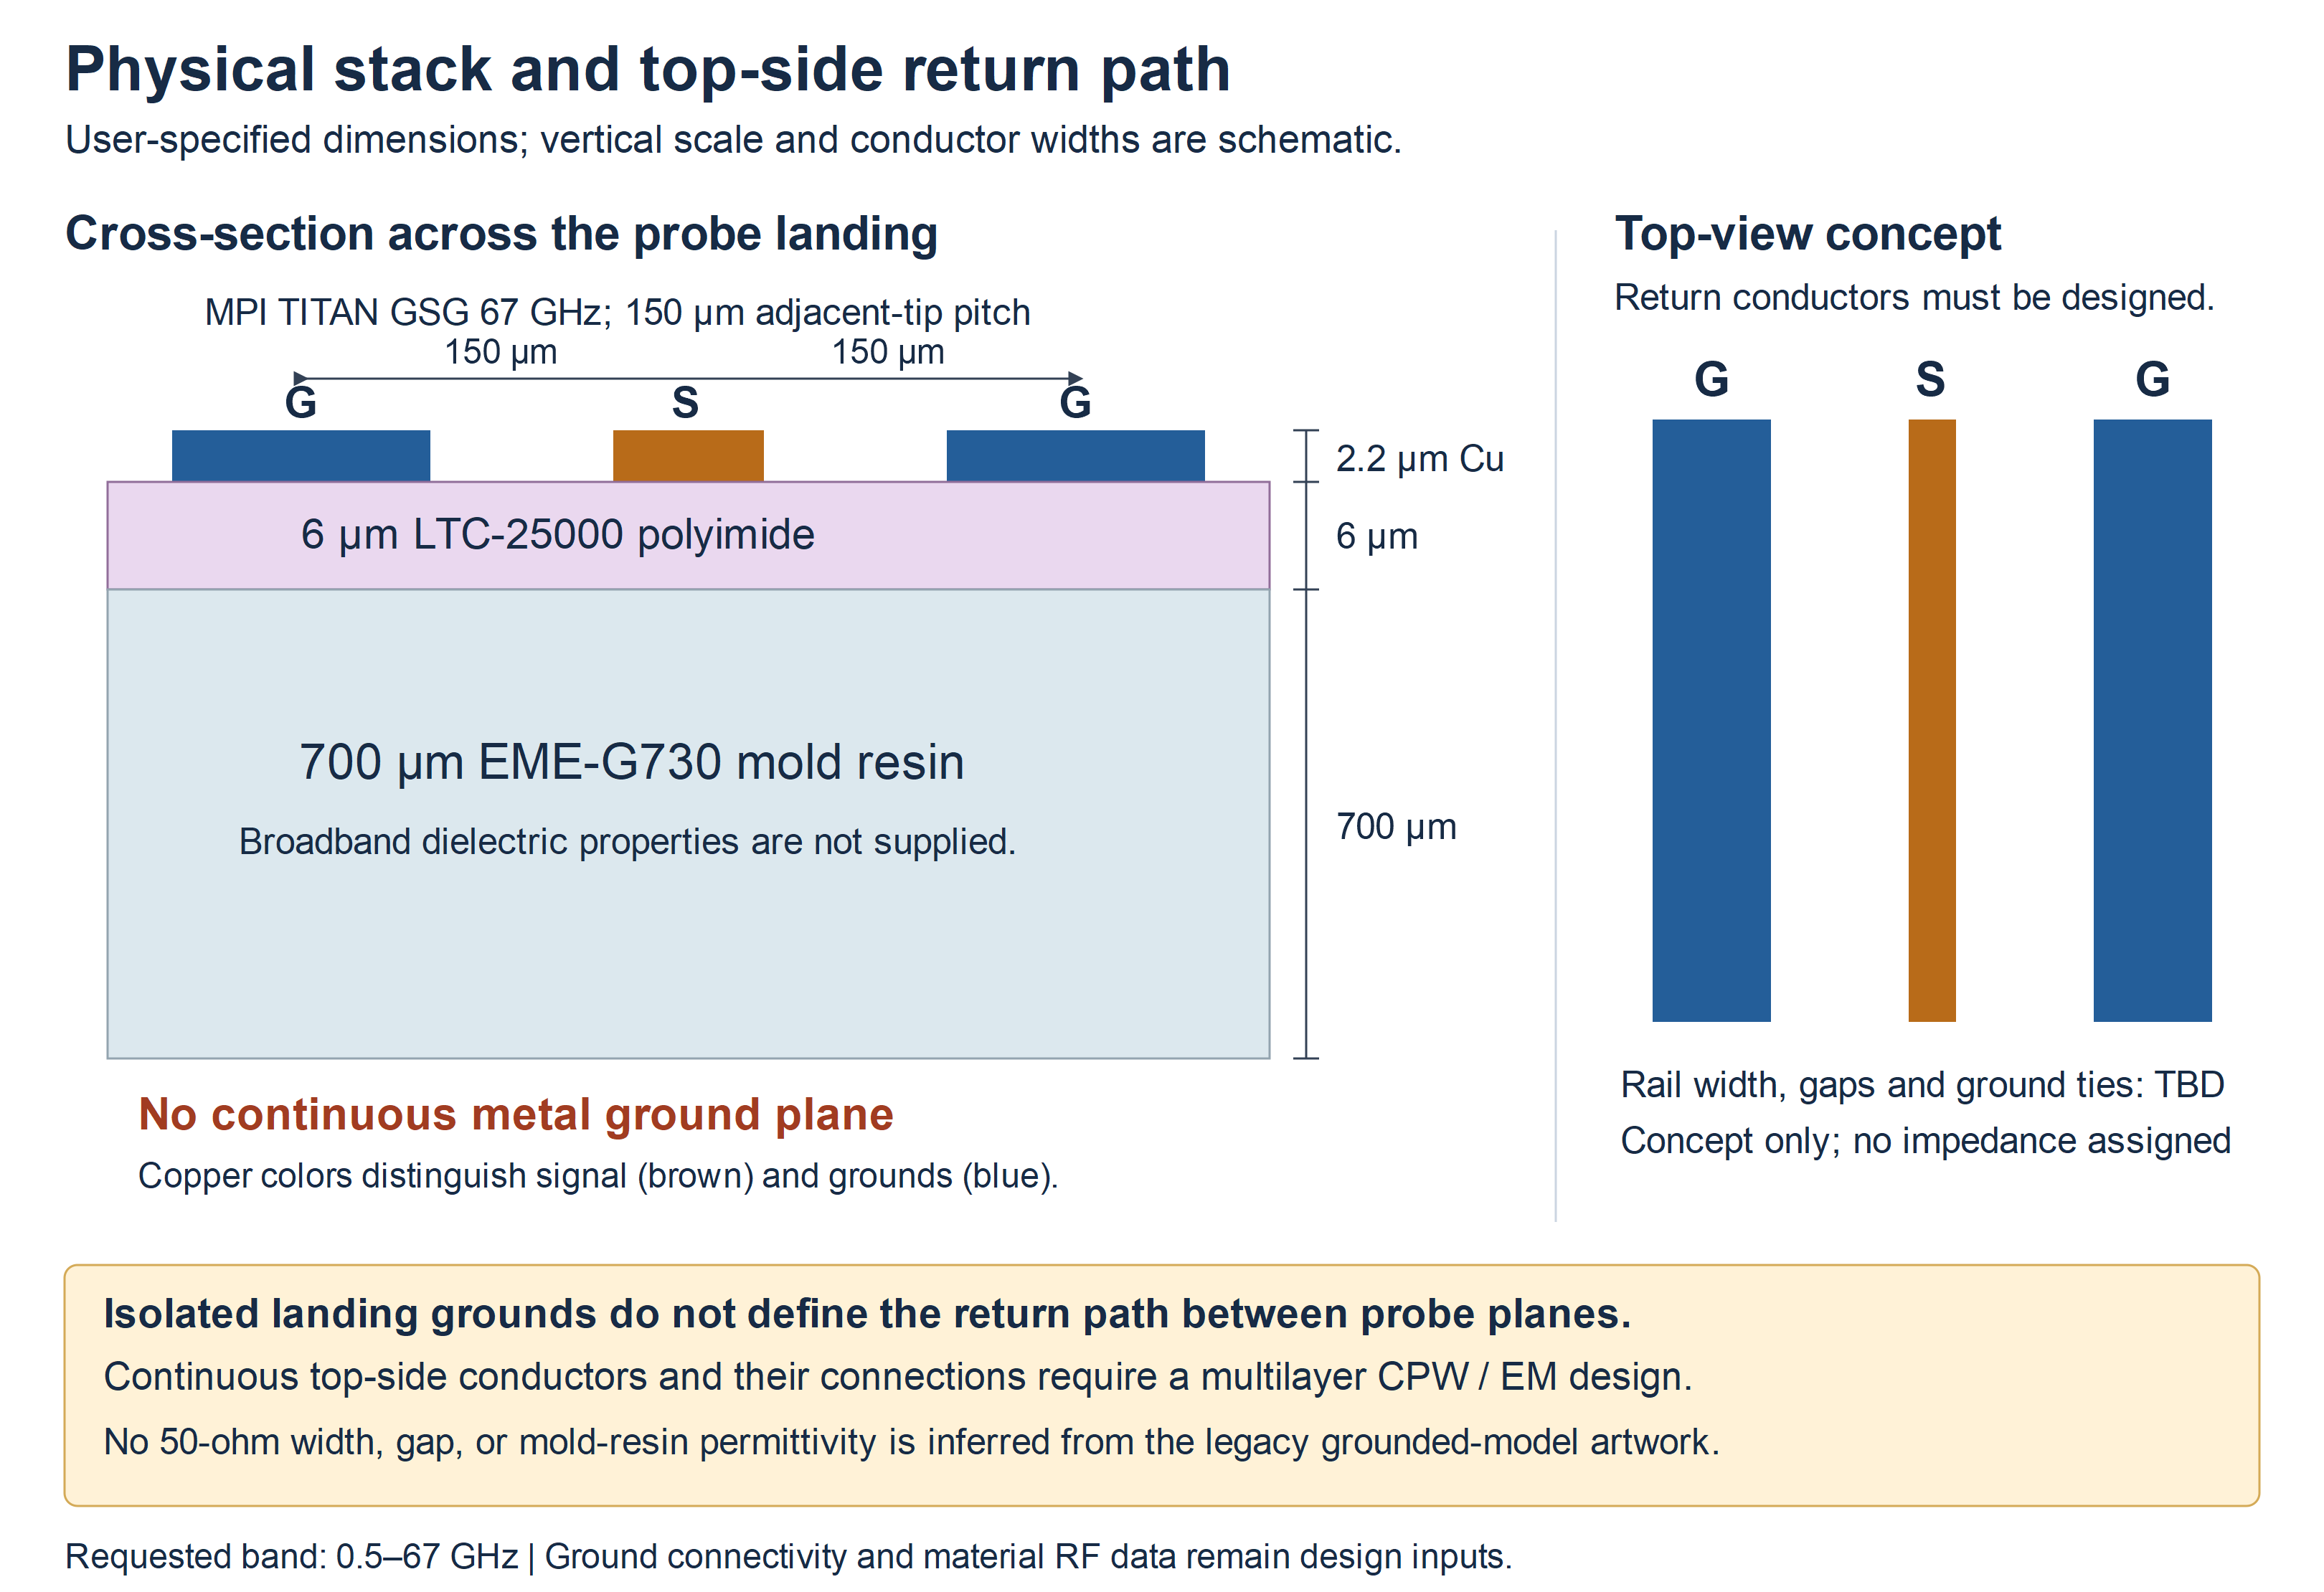
\includegraphics[width=.99\linewidth,height=.46\textheight,keepaspectratio]{assets/physical-stack.png}\end{center}
The physical structure is a two-dielectric, top-conductor configuration. Coplanar-waveguide fields occupy air, polyimide and mold resin. A 6 \ensuremath{\mu\mathrm{m}} polyimide coating cannot be substituted for the complete CPW substrate or for a 6 \ensuremath{\mu\mathrm{m}} distance to an absent ground plane. A prober chuck or support underneath the mold may also affect the boundary conditions and belongs in the final model.
\subhead{Connected ground conductors are required}
The revised BASIC drawings connect ground rails to the probe grounds and follow straight lines, bends and stub junctions. The ring has two outer half-ring returns connected to the launch banks, without an isolated inner ground island. These are schematic connectivity corrections, not synthesized CPW dimensions. Define physical widths and slots and model the bends, junctions and any required ground bonds or bridges without shorting the signal.
\subhead{Material properties remain open inputs}
\par\noindent\begin{tabular}{@{}p{.29\linewidth}p{.66\linewidth}@{}}\toprule
LTC-25000 & Grade identified in public process work [2]; verified 0.5--67 GHz Dk/Df not located.\\
EME-G730 & Exact suffix and RF data remain unspecified. Manufacturer G730 Ver. GR information concerns process/mechanical properties [3].\\
Reference calculations & Constant er=3.3 and loss tangent=0.01 are illustrative polyimide assumptions only. No mold Dk or Df was assigned.\\\bottomrule
\end{tabular}\par
The manufacturer's Dk/Df shown for G314 at 1 MHz are for a different grade and frequency. They are not used for EME-G730. Qucs distinguishes the CPW topology from microstrip and includes finite-substrate and conductor-thickness effects [4,5]; a stack-aware CPW or full-wave model is required here.

\newpage
\pageTitle{Reference relations}{Closed-form models shared by the coupons. Each relation was re-implemented and compared with the stored results when this report was built.}
\callout{\textbf{Scope.} These are the legacy reference models: a homogeneous microstrip over a continuous plane under the 6 \ensuremath{\mu\mathrm{m}} polyimide, with $\varepsilon_r=3.3$ and $\tan\delta=0.01$. They describe the ground-plane GDSII unit cells and the grounded reference curves. They do not describe the as-supplied stack, which has no plane.}
\subhead{Microstrip synthesis and effective permittivity}
With $u=W/h$ and $t'=T/h$, the thickness-corrected widths are
\[ \Delta u_1=\frac{t'}{\pi}\ln\!\left[1+\frac{4e\,\tanh^2\!\sqrt{6.517\,u}}{t'}\right],\qquad \Delta u_r=\Delta u_1\,\frac{1+\operatorname{sech}\sqrt{\varepsilon_r-1}}{2},\qquad u_1=u+\Delta u_1,\quad u_r=u+\Delta u_r. \]
The air-filled impedance and static effective permittivity are
\[ Z_{air}(u)=\frac{\eta_0}{2\pi}\ln\!\left[\frac{f(u)}{u}+\sqrt{1+\frac{4}{u^2}}\right],\qquad f(u)=6+(2\pi-6)\exp\!\left[-\left(\frac{30.666}{u}\right)^{0.7528}\right], \]
\[ \varepsilon_{eff}(u)=\frac{\varepsilon_r+1}{2}+\frac{\varepsilon_r-1}{2}\left(1+\frac{10}{u}\right)^{-ab},\qquad b=0.564\left(\frac{\varepsilon_r-0.9}{\varepsilon_r+3}\right)^{0.053}, \]
\[ a=1+\frac{1}{49}\ln\frac{u^4+(u/52)^2}{u^4+0.432}+\frac{1}{18.7}\ln\!\left[1+\left(\frac{u}{18.1}\right)^3\right]. \]
The reported impedance and thickness-corrected permittivity are
\[ Z_0=\frac{Z_{air}(u_r)}{\sqrt{\varepsilon_{eff}(u_r)}},\qquad \varepsilon_{eff,t}=\varepsilon_{eff}(u_r)\left[\frac{Z_{air}(u_1)}{Z_{air}(u_r)}\right]^{2},\qquad \eta_0=376.7303\ \Omega. \]
A 30-step bisection on $W\in[0.01h,100h]$ finds the width with $Z_0=50\ \Omega$. For $\varepsilon_r=3.3$, $h=6\,\mu\mathrm{m}$ and $T=2.2\,\mu\mathrm{m}$ this gives $u=2.0719$, $t'=0.3667$, $\Delta u_1=0.3992$, $\Delta u_r=0.2832$, $a=0.9998$, $b=0.5359$, $W=12.431\,\mu\mathrm{m}$, $\varepsilon_{eff,t}=2.4765$.
The model is static. The Getsinger dispersion corner, $f_p=Z_0/(2\mu_0 h)=3.32$ THz, lies far above the 67 GHz band edge, so frequency-independent $Z_0$ and $\varepsilon_{eff}$ are reasonable for a 6 \ensuremath{\mu\mathrm{m}} dielectric over a plane.
\subhead{Phase, delay and reflection}
\[ v_p=\frac{c}{\sqrt{\varepsilon_{eff}}}=190.5\ \mathrm{mm/ns},\qquad \tau=\frac{\ell\sqrt{\varepsilon_{eff}}}{c},\qquad \theta=\frac{360^\circ f\,\ell\sqrt{\varepsilon_{eff}}}{c},\qquad \lambda_g=\frac{c}{f\sqrt{\varepsilon_{eff}}}. \]
At 5 GHz $\lambda_g=38.101$ mm; at 67 GHz $\lambda_g=2.843$ mm and the delay is 5.249 ps/mm. A mismatch to the $Z_0=50\ \Omega$ reference gives
\[ \Gamma=\frac{Z-Z_0}{Z+Z_0},\qquad \mathrm{RL}=-20\log_{10}|\Gamma|,\qquad \mathrm{IL}=-20\log_{10}|S_{21}|. \]
\subhead{Conductor and dielectric attenuation}
With resistivity $\rho$, RMS roughness $\Delta$ and loss tangent $\tan\delta$,
\[ \delta_s=\sqrt{\frac{\rho}{\pi f\mu_0}},\quad R_s=\sqrt{\pi f\mu_0\rho},\quad K_r=1+\frac{2}{\pi}\arctan\!\left[1.4\left(\frac{\Delta}{\delta_s}\right)^{2}\right],\quad K_i=\exp\!\left[-1.2\left(\frac{Z_0}{\eta_0}\right)^{0.7}\right], \]
\[ \alpha_c=8.686\,\frac{R_s}{Z_0W}\,K_rK_i,\qquad \alpha_d=8.686\,\frac{\pi f}{c}\,\frac{\varepsilon_r}{\sqrt{\varepsilon_{eff}}}\,\frac{\varepsilon_{eff}-1}{\varepsilon_r-1}\tan\delta,\qquad \alpha=\alpha_c+\alpha_d\quad[\mathrm{dB\ per\ unit\ length}]. \]
Here $\rho=17.2\ \mathrm{n\Omega\,m}$ and $\Delta=0.3\,\mu\mathrm{m}$. The roughness factor $K_r$ rises from 1 toward 2 as $\delta_s$ falls below $\Delta$. The expression assumes a conductor thick compared with $\delta_s$. At low frequency, where $\delta_s>T$, current fills the 2.2 \ensuremath{\mu\mathrm{m}} copper and the loss approaches the dc limit $\alpha_{dc}=8.686\,R'_{dc}/(2Z_0)$ with $R'_{dc}=\rho/(WT)$.
\subhead{What each coupon returns}
{\small
\par\noindent\begin{tabular}{@{}p{.15\linewidth}p{.20\linewidth}p{.25\linewidth}p{.33\linewidth}@{}}\toprule
Structure & Measurement & Raw data & Extracted result\\\midrule
RDLLOSS & 2-port, 3 lines & $S_{21}$ of each length & attenuation $\alpha(f)$ from $\Delta\mathrm{IL}/\Delta L$\\
RDXTALK & 4-port & $S_{21},S_{31},S_{41}$ vs gap & coupling, $Z_e$, $Z_o$, $\varepsilon_e$, $\varepsilon_o$\\
RFLEAK & 2-port + dc & $S_{21}$, $S_{11}$, $R_{dc}$ & layer-transition loss and reflection\\
STUBTEST & 3-port; P3 north & $S_{21}$ with external P3 open/short & $\varepsilon_{eff}$ and stub end effect\\
TRLSET & 2-port standards & thru, lines, reflect & $\gamma$, $\varepsilon_{eff}$, reference planes\\
VIAMATCH & 1-port & $S_{11}$ of bare and matched & $Z_{in}$, return loss, tolerance\\
ZCOUPON & 2-port & $S_{11}$, TDR step, delay & $Z_0$ and $\tau$ versus width\\
RESONATOR2 & 2-port & $S_{21}$ resonance peaks & $f_n$, $Q$, $\varepsilon_{eff}$, $\alpha$\\\bottomrule
\end{tabular}\par

}

\newpage
\pageTitle{RDLLOSS / differential line loss}{Two ports: P1 west, P2 east; north/south parked.}
\callout{\textbf{Source artwork only.} Native numerical labels below belong to the legacy grounded reference and do not establish electrical behavior on the supplied ungrounded stack.}
\preview{rdlloss}{Actual native drawing commands; the printed delta length is a hypothetical grounded-model result.}
\subhead{Measurement concept}
Three separate coupons use common launches and short, middle and long line lengths. The intended measurement is the change in attenuation with length.

\minihead{Governing relations}
Three lines of identical cross section differ only in length. Launches, pads and ground transitions are common to all three and cancel when insertion losses $\mathrm{IL}_i(f)=-20\log_{10}|S_{21,i}|$ are subtracted:
\[ \alpha(f)\simeq\frac{\mathrm{IL}_L(f)-\mathrm{IL}_S(f)}{L_L-L_S}\ \ [\mathrm{dB/mm}],\qquad \alpha=\alpha_c+\alpha_d\quad\text{(Reference relations)}. \]
The long-line increment is sized so that the loss difference at the top of the band equals a chosen value $\mathrm{IL}_\Delta$:
\[ \Delta L=\frac{\mathrm{IL}_\Delta}{\alpha(f_{max})},\qquad L_M=L_S+\tfrac12\Delta L,\qquad L_L=L_S+\Delta L. \]
\minihead{Worked reference values}
At $f_{max}=67$ GHz $\alpha_c=1.194$ and $\alpha_d=0.0821$ dB/mm, so $\alpha=1.2765$ dB/mm and the conductor supplies 93.6\% of the loss. For $\mathrm{IL}_\Delta=0.5$ dB, $\Delta L=0.5/1.2765=0.3917$ mm and the three lines are $L_S=2.000$, $L_M=2.196$ and $L_L=2.392$ mm.
The dc limit is $R'_{dc}=\rho/(WT)=0.629\ \Omega/\mathrm{mm}$, giving $\alpha_{dc}=0.0546$ dB/mm, close to the $0.0620$ dB/mm the model returns at 0.5 GHz. The skin depth equals the 2.2 \ensuremath{\mu\mathrm{m}} thickness at $f=\rho/(\pi\mu_0T^2)=0.90$ GHz, and $3\delta_s\le T$ only above $8.10$ GHz, which is where the thick-conductor assumption becomes valid.
\minihead{Expected test data}
Each line gives a smooth $S_{21}$ that falls with frequency. The three curves are parallel and spaced by $\alpha\,\Delta L/2$. The difference $\Delta\mathrm{IL}(f)$ rises from $0.024$ dB at 0.5 GHz to $0.500$ dB at 67 GHz. Growth is close to $\sqrt f$ in mid-band (conductor) with a smaller term linear in $f$ (dielectric). Below about $0.9$ GHz the curve flattens toward the dc limit. The 0.5 GHz difference of a few hundredths of a dB is comparable to the repeatability of a calibrated VNA trace, so low-frequency points should be averaged or fitted to the $\sqrt f$ plus $f$ form rather than read directly. The longest line is $0.84$ guided wavelengths at 67 GHz, so a mismatch ripple appears on $S_{11}$ if the launch is not 50 $\Omega$.
\par\noindent\begin{tabular}{@{}rrrrrrrr@{}}\toprule
$f$ (GHz) & $\delta_s$ ($\mu$m) & $\alpha_c$ & $\alpha_d$ & $\alpha$ & IL short & IL long & $\Delta$IL\\\midrule
0.5 & 2.952 & 0.0614 & 0.0006 & 0.0620 & 0.124 & 0.148 & 0.0243\\
1.0 & 2.087 & 0.0876 & 0.0012 & 0.0888 & 0.178 & 0.212 & 0.0348\\
5.0 & 0.933 & 0.2099 & 0.0061 & 0.2160 & 0.432 & 0.517 & 0.0846\\
10.0 & 0.660 & 0.3207 & 0.0123 & 0.3330 & 0.666 & 0.796 & 0.1304\\
20.0 & 0.467 & 0.5130 & 0.0245 & 0.5375 & 1.075 & 1.286 & 0.2105\\
40.0 & 0.330 & 0.8410 & 0.0490 & 0.8900 & 1.780 & 2.129 & 0.3486\\
67.0 & 0.255 & 1.1944 & 0.0821 & 1.2765 & 2.553 & 3.053 & 0.5000\\\bottomrule
\end{tabular}\par

{\footnotesize Attenuation columns in dB/mm; IL columns in dB for the 2.000 mm and 2.392 mm lines; $\Delta$IL is long minus short.}
\response{rdlloss-response}{Reference conductor, dielectric and total loss versus frequency (grounded reference model).}

\subhead{Changes needed for the supplied stack}
The sketch now connects top-side ground rails along each line. Replace microstrip width and attenuation synthesis with ungrounded multilayer CPW and size the rails, slots and identical transitions. Include copper thickness, roughness, both dielectric losses, mismatch and calibration.
\textbf{Specific model limit.} The source loss approximation also assumes a thick conductor. At 500 MHz its hypothetical skin depth is about 2.952 \ensuremath{\mu\mathrm{m}}, exceeding the 2.2 \ensuremath{\mu\mathrm{m}} copper thickness. Its three-skin-depth condition is reached only above about 8.102 GHz.

\newpage
\pageTitle{RDXTALK / four-port crosstalk}{P1 west, P2 north, P3 south, P4 east. Aggressor W-to-N; victim S-to-E.}
\callout{\textbf{Source artwork only.} Native numerical labels below belong to the legacy grounded reference and do not establish electrical behavior on the supplied ungrounded stack.}
\preview{rdxtalk}{Four cardinal GSG landings with connected outer grounds and no signal crossover. The coupled pair retains an unshielded central gap.}
\subhead{Measurement concept}
Preserve the two parallel coupled conductors and cardinal access fanouts. P1 drives the aggressor; P2 is through, P3 is near-end and P4 is far-end coupling.

\minihead{Governing relations}
The two adjacent conductors are resolved into even and odd modes with impedances $Z_e,Z_o$ and permittivities $\varepsilon_e,\varepsilon_o$. For a section of length $\ell$ in a $Z_0$ system, each mode $m\in\{e,o\}$ has electrical length $\theta_m=2\pi f\ell\sqrt{\varepsilon_m}/c$ and
\[ T_m=\frac{2}{2\cos\theta_m+j\!\left(\frac{Z_m}{Z_0}+\frac{Z_0}{Z_m}\right)\sin\theta_m},\qquad \Gamma_m=\frac{j\!\left(\frac{Z_m}{Z_0}-\frac{Z_0}{Z_m}\right)\sin\theta_m}{2\cos\theta_m+j\!\left(\frac{Z_m}{Z_0}+\frac{Z_0}{Z_m}\right)\sin\theta_m}. \]
The four-port parameters (P1 aggressor near, P2 aggressor far, P3 victim near, P4 victim far) follow from superposition:
\[ S_{11}=\tfrac12(\Gamma_e+\Gamma_o),\quad S_{21}=\tfrac12(T_e+T_o),\quad S_{31}=\tfrac12(\Gamma_e-\Gamma_o),\quad S_{41}=\tfrac12(T_e-T_o). \]
The mode data are recovered from a measurement by the inverse relations $\Gamma_e=S_{11}+S_{31}$, $\Gamma_o=S_{11}-S_{31}$, $T_e=S_{21}+S_{41}$ and $T_o=S_{21}-S_{41}$. The coupling coefficient is $k_c=(Z_e-Z_o)/(Z_e+Z_o)$. Near-end coupling needs only $Z_e\ne Z_o$. Far-end coupling needs a velocity difference $\varepsilon_e\ne\varepsilon_o$ or a mismatch, because the two modes then arrive with different phase.
\minihead{Worked reference values}
For the 20 \ensuremath{\mu\mathrm{m}} gap, $Z_e=21.996\ \Omega$, $Z_o=20.890\ \Omega$, $\varepsilon_e=2.963$, $\varepsilon_o=2.799$, so $k_c=0.0258$ and $\sqrt{Z_eZ_o}=21.44\ \Omega$. Over the 5.0 mm coupled length at 67 GHz, $\theta_e-\theta_o=19.5^\circ$. The first quarter-wave of the even mode occurs near $8.71$ GHz.
\minihead{Expected test data}
At low frequency $S_{31}$ and $S_{41}$ rise at 20 dB per decade, which is 6 dB per octave. For the 20 \ensuremath{\mu\mathrm{m}} gap $S_{31}$ moves from $-54.3$ dB at 0.5 GHz to $-48.5$ dB at 1 GHz. Coupling flattens and ripples once the coupled section is about a quarter wavelength, near 9 GHz, then continues to rise to $-17.6$ dB (near end) and $-15.5$ dB (far end) at 67 GHz. Doubling the gap lowers low-frequency coupling by about 6.5 dB per step ($-47.8$, $-54.3$, $-60.8$ dB at 0.5 GHz for 10, 20, 40 \ensuremath{\mu\mathrm{m}}).
The through path is not a flat 0 dB. The coupled lines are about 21 $\Omega$, so the 50 $\Omega$ ports see a mismatch and $S_{21}$ dips to $-2.71$ dB at 10 GHz and $-1.40$ dB at 67 GHz in this lossless model. A real device adds conductor loss on top.
\par\noindent\begin{tabular}{@{}r*{3}{r}*{3}{r}r@{}}\toprule
$f$ (GHz) & $S_{31}$ 10 & $S_{31}$ 20 & $S_{31}$ 40 & $S_{41}$ 10 & $S_{41}$ 20 & $S_{41}$ 40 & $S_{21}$ 20\\\midrule
0.5 & $-47.8$ & $-54.3$ & $-60.8$ & $-56.9$ & $-67.1$ & $-73.2$ & $-0.03$\\
1.0 & $-42.1$ & $-48.5$ & $-55.1$ & $-50.8$ & $-60.3$ & $-66.6$ & $-0.12$\\
5.0 & $-33.6$ & $-39.5$ & $-46.1$ & $-36.1$ & $-41.7$ & $-48.4$ & $-1.89$\\
10.0 & $-28.7$ & $-33.4$ & $-40.1$ & $-28.8$ & $-33.4$ & $-40.1$ & $-2.71$\\
20.0 & $-27.0$ & $-30.2$ & $-37.1$ & $-22.4$ & $-25.9$ & $-32.7$ & $-0.61$\\
40.0 & $-22.0$ & $-25.4$ & $-32.2$ & $-19.2$ & $-22.8$ & $-29.7$ & $-1.75$\\
67.0 & $-14.0$ & $-17.6$ & $-24.3$ & $-11.8$ & $-15.5$ & $-22.2$ & $-1.40$\\\bottomrule
\end{tabular}\par

{\footnotesize Columns in dB; the numbers 10, 20 and 40 are the gap in $\mu$m. $S_{21}$ is for the 20 $\mu$m gap.}
\response{rdxtalk-response}{Reference near-end, far-end and through response for the three gaps (grounded reference model).}

\subhead{Changes needed for the supplied stack}
Define the top-ground layout before solving the coupled CPW modes. Ground rails, slots, corners and finite ground regions all affect coupling. Use a four-port multilayer EM model and calibrate all four probe planes.
\textbf{Specific model limit.} The current coupled microstrip calculation uses zero-thickness DUT conductors and omits access bends and probe parasitics. Its 1 mm adjacent landing-centre rule is adjustable and does not establish mechanical clearance of the installed probe bodies.

\smallskip\textbf{Port meaning:} S21 is W-to-N aggressor through, S31 is W-to-S near-end coupling, and S41 is W-to-E far-end coupling. Full four-port calibration is required.

\newpage
\pageTitle{RFLEAK / via-connected layer transition}{Two top-side ports: P1 west, P2 east; north/south parked.}
\callout{\textbf{Source artwork only.} Native numerical labels below belong to the legacy grounded reference and do not establish electrical behavior on the supplied ungrounded stack.}
\preview{rfleak}{Top view: connected G-S-G routing and via locations. Signal side view: upper-left L1 drops to lower-right L2, then returns to L1 at the east pads. Not to scale.}
\subhead{Measurement concept}
The west trace is on upper layer L1. A central signal via joins it to the right-hand trace on lower layer L2. Separate G-S-G vias at the east end return all three conductors to the top-side probe pads. Ground rails follow the traces and have their own layer transitions.

\minihead{Governing relations}
The drawn coupon is a connected path: M2 pads and feeds, a 4 mm M1 line, and V1 transitions at each end with ground vias at $\pm150\,\mu\mathrm{m}$. Its direct-current resistance and the series impedance of the two transitions are
\[ R_{dc}=\frac{\rho\,\ell}{WT}+2R_v,\qquad R_v=\frac{\rho h_v}{\pi r_v^2},\qquad L_v=\frac{\mu_0h_v}{2\pi}\ln\frac{b}{r_v},\qquad Z_s=2\,(R_v+j\omega L_v), \]
\[ S_{21}=\frac{2Z_0}{2Z_0+Z_s},\qquad S_{11}=\frac{Z_s}{2Z_0+Z_s}. \]
Here $r_v$ is the via radius and $b$ is the distance to the return via; $L_v$ is the coaxial estimate used by the VIAMATCH surrogate. The line itself adds $\mathrm{IL}=\alpha(f)\,\ell$ from the Reference relations.
The legacy isolated-plate model, kept for comparison, treats the overlap as a series capacitor:
\[ C=\frac{\varepsilon_0\varepsilon_rO_WO_L}{g},\qquad X=4\pi fZ_0C,\qquad |S_{21}|=\frac{X}{\sqrt{1+X^2}}. \]
\minihead{Worked reference values}
No second-metal separation is defined, so $h_v=6\,\mu\mathrm{m}$ is assumed. With $r_v=20\,\mu\mathrm{m}$ and $b=150\,\mu\mathrm{m}$: $R_v=82.1\ \mu\Omega$ and $L_v=2.42$ pH, so the pair of transitions adds $X=2.04\ \Omega$ at 67 GHz. The signal path is about $4\ \mathrm{mm}$ of M1 plus $2\times0.5\ \mathrm{mm}$ of M2 feed, $\ell=5$ mm, so $R_{dc}\approx3.14\ \Omega$ if M2 has the same width and thickness as M1. For the plate model, $C=0.03896$ pF for the $80\times100\ \mu\mathrm{m}$ overlap and a 6 \ensuremath{\mu\mathrm{m}} gap, and $|S_{21}|$ reaches the 40 dB target only for $C\le0.238$ fF.
\minihead{Expected test data}
For the drawn path the measured $S_{21}$ is a low-loss through response. It follows the line loss with a small extra drop from the transitions, and $S_{11}$ stays well below $-30$ dB until the vias become electrically large. A dc four-wire measurement between the signal pads should read a few ohms and confirms continuity of both V1 transitions. A single via has under $0.1$ m$\Omega$ here, so a via chain or a through coupon without vias is needed to resolve it. Comparing against a no-via through line of the same length isolates the transition: any $\Delta S_{21}$ beyond a few hundredths of a dB indicates an unexpected via resistance or a layer-to-layer dielectric gap.
\par\noindent\begin{tabular}{@{}rrrr@{}}\toprule
$f$ (GHz) & line IL, 5 mm (dB) & via pair $S_{21}$ (dB) & via pair $S_{11}$ (dB)\\\midrule
0.5 & 0.310 & $0.0000$ & $-76.4$\\
1.0 & 0.444 & $0.0000$ & $-70.3$\\
5.0 & 1.080 & $0.0000$ & $-56.4$\\
10.0 & 1.665 & $-0.0001$ & $-50.3$\\
20.0 & 2.688 & $-0.0002$ & $-44.3$\\
40.0 & 4.450 & $-0.0007$ & $-38.3$\\
67.0 & 6.382 & $-0.0018$ & $-33.8$\\\bottomrule
\end{tabular}\par

The reference isolated-plate model gives the opposite behaviour: a capacitive isolation that falls from tens of dB toward 0 dB as frequency rises.
\par\noindent\begin{tabular}{@{}rrrr@{}}\toprule
$f$ (GHz) & $S_{21}$, 0.5$\times$ area & $S_{21}$, 1$\times$ area & $S_{21}$, 2$\times$ area\\\midrule
0.5 & $-44.27$ & $-38.25$ & $-32.23$\\
1.0 & $-38.25$ & $-32.23$ & $-26.21$\\
5.0 & $-24.28$ & $-18.31$ & $-12.48$\\
10.0 & $-18.31$ & $-12.48$ & $-7.14$\\
20.0 & $-12.48$ & $-7.14$ & $-3.10$\\
40.0 & $-7.14$ & $-3.10$ & $-1.01$\\
67.0 & $-3.96$ & $-1.37$ & $-0.39$\\\bottomrule
\end{tabular}\par

{\footnotesize $S_{21}$ in dB for the legacy plate model. Doubling the overlap area doubles $C$ and raises $S_{21}$ by 6 dB at low frequency.}
\response{rfleak-response}{Legacy isolated-plate leakage versus frequency for three overlap areas. It is not the response of the drawn via-connected path.}

\subhead{Changes needed for the supplied stack}
Confirm the second patterned metal layer and define its thickness and dielectric separation. Size the signal and ground vias, rails and slots using a multilayer EM model. This connected structure is not an isolated broadside leakage capacitor.
\textbf{Specific model limit.} The retained numerical routines calculate coupling between isolated plates, not this via-connected path. Their capacitance, isolation and via-fence rules must not be interpreted as the response of the new drawing.

\newpage
\pageTitle{STUBTEST / three-port shunt stubs}{Three ports: P1 west, P2 east, P3 north at the shunt-branch end.}
\callout{\textbf{Source artwork only.} Native numerical labels below belong to the legacy grounded reference and do not establish electrical behavior on the supplied ungrounded stack.}
\preview{stubtest}{Three-port source artwork with P1 west, P2 east and north-facing P3 at the shunt branch end.}
\subhead{Measurement concept}
A shunt branch connects the P1-P2 through line to an accessible north-facing P3 GSG port. For two-port reference sweeps, P3 is externally left open or terminated in a short.

\minihead{Governing relations}
A shunt stub of impedance $Z_s$ and electrical length $\theta_s=2\pi f\ell_{eff}\sqrt{\varepsilon_s}/c$ loads the through line with
\[ Y_{open}=j\,\frac{\tan\theta_s}{Z_s},\qquad Y_{short}=-j\,\frac{\cot\theta_s}{Z_s},\qquad S_{21}=\frac{2}{2+Z_0Y_{in}}, \]
\[ \mathrm{IL}_{open}=10\log_{10}\!\left[1+\left(\frac{Z_0\tan\theta_s}{2Z_s}\right)^{2}\right],\qquad \mathrm{IL}_{short}=10\log_{10}\!\left[1+\left(\frac{Z_0\cot\theta_s}{2Z_s}\right)^{2}\right]. \]
An open stub notches where $\theta_s=(2k-1)\pi/2$; a short stub notches where $\theta_s=k\pi$:
\[ \ell_{open}=\frac{c}{4f_c\sqrt{\varepsilon_s}}-\Delta\ell,\qquad \ell_{short}=\frac{c}{2f_c\sqrt{\varepsilon_s}},\qquad f_k=(2k-1)\,f_c\ \ (\text{open}). \]
The open-end extension is $\Delta\ell=0.412\,h\,\dfrac{(\varepsilon_s+0.3)(u_s+0.264)}{(\varepsilon_s-0.258)(u_s+0.8)}$ with $u_s=W_s/h$. STUBTEST exposes the branch end as P3 north; open and short are external P3 terminations, not fixed DUT connections. A lossy stub does not null completely. With stub attenuation $\alpha_s$ in Np per unit length, $Y_{open}$ at resonance is $\coth(\alpha_s\ell)/Z_s$, so the notch depth is
\[ S_{21,min}=\frac{2}{2+\dfrac{Z_0}{Z_s}\coth(\alpha_s\ell)}. \]
\minihead{Worked reference values}
A $70\ \Omega$ stub gives $W_s=6.221\,\mu\mathrm{m}$, $\varepsilon_s=2.3119$ and $\Delta\ell=2.226\,\mu\mathrm{m}$. For $f_c=20$ GHz, $\ell=2.46459-0.002226=2.46236$ mm. The stub is much narrower than the 50 $\Omega$ line, so its loss is larger: $\alpha_s=0.700$ dB/mm at 20 GHz from the Reference relations, which limits the nominal notch to $S_{21,min}=-9.0$ dB instead of $-\infty$.
\minihead{Expected test data}
$S_{21}$ is near 0 dB at low frequency, then shows a sharp notch at $f_1$ and a second notch at $3f_1$, both inside the 0.5 to 67 GHz band. The three stubs move the notch by the inverse of their length ($\pm10\%$ length gives $\mp10\%$ frequency). The product $f_1\ell_{eff}$ should be the same for all three stubs and equals $c/(4\sqrt{\varepsilon_s})=49.29$ GHz\,mm, so any spread shows an error in the stub end effect rather than in $\varepsilon_{eff}$. A measurement of $f_1$ gives $\varepsilon_s=[c/(4f_1\ell_{eff})]^2$. The measured notch will be around $-9$ dB deep, not the 120 dB cap of the ideal calculation, because stub loss limits it. The retained source sweep is a two-port P1-to-P2 response with P3 externally open or shorted; it does not produce the full three-port S matrix.
\par\noindent\begin{tabular}{@{}lrrrrrr@{}}\toprule
Stub & $\ell$ (mm) & $f_1$ (GHz) & $3f_1$ (GHz) & $f_1\ell_{eff}$ & IL at 10 GHz & IL at 67 GHz\\\midrule
0.9$\times$ length & 2.216 & 22.22 & 66.66 & 49.29 & $0.39$ & $23.46$\\
1$\times$ length & 2.462 & 20.00 & 60.00 & 49.29 & $0.52$ & $1.27$\\
1.1$\times$ length & 2.709 & 18.18 & 54.55 & 49.29 & $0.70$ & $0.16$\\\bottomrule
\end{tabular}\par

{\footnotesize IL in dB from the lossless stub model; $f_1\ell_{eff}$ in GHz mm.}
\response{stubtest-response}{Reference through loss of the open stub for 0.9, 1.0 and 1.1 times the nominal length (grounded reference model).}

\subhead{Changes needed for the supplied stack}
Design the through line, branch, tee junction and all three GSG ground returns as CPW on the actual two-dielectric stack. Keep P3 accessible for calibrated three-port measurements; apply open/short conditions externally at its reference plane.
\textbf{Specific model limit.} The native 70 ohm stub synthesis and 20 GHz notch example use the grounded microstrip reference. The retained response sweep calculates the P1-P2 response with P3 externally open or shorted; it does not calculate the full three-port S matrix or establish physical CPW behavior.

The gallery also contains \texttt{stubtest-short.png}. Both artworks retain the same three accessible ports; open or short is an external P3 test condition.

\newpage
\pageTitle{TRLSET / multiline calibration standards}{Two ports: P1 west, P2 east; one standard measured at a time.}
\callout{\textbf{Source artwork only.} Native numerical labels below belong to the legacy grounded reference and do not establish electrical behavior on the supplied ungrounded stack.}
\preview{trlset}{Native schematic of separate standards; row spacing and drawn lengths are illustrative and not a mask layout.}
\subhead{Measurement concept}
The standards retain a common cross section and launches, with a thru and several extra line lengths. The same reflect reference is used across measurements.

\minihead{Governing relations}
Multiline TRL measures several lines of known length differences and recovers the propagation constant $\gamma=\alpha+j\beta$. Line $j$ is centred where its length difference from the thru is a quarter wavelength, and the centres are spaced geometrically across the band:
\[ f_{c,j}=F_1\left(\frac{F_2}{F_1}\right)^{\frac{j-1}{N_L-1}},\qquad \Delta L_j=\frac{c}{4f_{c,j}\sqrt{\varepsilon_{eff}}},\qquad L_j=L_{thru}+\Delta L_j. \]
A pair $(i,j)$ is usable when its phase difference lies between $20^\circ$ and $160^\circ$, and the calibration error grows roughly as $1/|\sin\Delta\theta|$:
\[ \Delta\theta_{ij}=\frac{360^\circ f\,|L_i-L_j|\sqrt{\varepsilon_{eff}}}{c},\qquad 20^\circ\le\Delta\theta_{ij}\le160^\circ. \]
The calibration solves for the eigenvalues of the line-thru transfer-matrix ratio, $\lambda=e^{-\gamma\Delta L}$, so
\[ \gamma=-\frac{\ln\lambda}{\Delta L},\qquad \varepsilon_{eff}=\left(\frac{\beta c}{2\pi f}\right)^{2}. \]
The reflect standard fixes the reference plane. For an open with end extension $\Delta\ell_o$, $\Gamma_{open}=e^{-j2\beta\Delta\ell_o}$ is within a few degrees of $+1$ at these dimensions.
\minihead{Worked reference values}
With $F_1=0.5$ GHz, $F_2=67$ GHz and $N_L=5$, the line centres are 0.50, 1.70, 5.79, 19.69, 67.00 GHz and the length differences are 95.25, 28.00, 8.23, 2.42, 0.71 mm. Line 1 would be 96.3 mm long, which exceeds the 40 mm limit, so it is dropped. The remaining pairs still cover all 201 logarithmically spaced points with 0 uncovered.
\minihead{Expected test data}
Every standard returns $|S_{21}|=e^{-\alpha L}$ with a phase ramp $-\beta L$ that wraps repeatedly across the band. After calibration the lines give a smooth $\varepsilon_{eff}\approx2.476$ and an $\alpha(f)$ curve matching the RDLLOSS coupon. The thru and the lines are only usable inside their phase windows, and outside them the extracted $\gamma$ becomes noisy. Because the longest line loses $37$ dB at 67 GHz, it is excluded there by the selection rule rather than by the VNA dynamic range. The open reflect shows $|S_{11}|\approx1$ with a phase that falls with frequency.
\par\noindent\begin{tabular}{@{}crrrcc@{}}\toprule
Line & $f_c$ (GHz) & $\Delta L$ (mm) & $L$ (mm) & usable $20^\circ$--$160^\circ$ (GHz) & fits\\\midrule
1 & 0.500 & 95.251 & 96.251 & 0.11--0.89 & no\\
2 & 1.701 & 27.996 & 28.996 & 0.38--3.02 & yes\\
3 & 5.788 & 8.228 & 9.228 & 1.29--10.29 & yes\\
4 & 19.692 & 2.418 & 3.418 & 4.38--35.01 & yes\\
5 & 67.000 & 0.711 & 1.711 & 14.89--119.11 & yes\\\bottomrule
\end{tabular}\par

\par\noindent\begin{tabular}{@{}rrrr@{}}\toprule
Line & $L$ (mm) & IL at $f_c$ (dB) & IL at 67 GHz (dB)\\\midrule
2 & 28.996 & 3.41 & 37.0\\
3 & 9.228 & 2.18 & 11.8\\
4 & 3.418 & 1.82 & 4.4\\
5 & 1.711 & 2.18 & 2.2\\\bottomrule
\end{tabular}\par

\par\noindent\begin{tabular}{@{}rcrr@{}}\toprule
$f$ (GHz) & pair & $\Delta\theta$ ($^\circ$) & $1/|\sin\Delta\theta|$\\\midrule
0.5 & 0--2 & 26.5 & 2.24\\
1.0 & 0--2 & 52.9 & 1.25\\
5.0 & 0--2 & 84.5 & 1.00\\
10.0 & 3--4 & 109.8 & 1.06\\
20.0 & 0--4 & 91.4 & 1.00\\
40.0 & 2--5 & 82.5 & 1.01\\
67.0 & 0--5 & 90.0 & 1.00\\\bottomrule
\end{tabular}\par

{\footnotesize The last table lists the pair the selection rule picks at each sample frequency.}
\response{trlset-response}{Pair phase difference across the band for the selected line pairs (grounded reference model).}

\subhead{Changes needed for the supplied stack}
Use the same connected CPW grounds, slots and stack as the DUTs. Choose line lengths from the actual dispersive propagation constant, then check pairwise phase and calibration conditioning across 0.5 to 67 GHz.
\textbf{Specific model limit.} The legacy source uses a homogeneous microstrip effective permittivity. Its two-port west/east standards do not supply the complete four-head calibration needed for the cardinal RDXTALK device.

\newpage
\pageTitle{VIAMATCH / one-port stud and via match}{One external port: P1 west. The RL/RX load is internal; east/north/south parked.}
\callout{\textbf{Source artwork only.} Native numerical labels below belong to the legacy grounded reference and do not establish electrical behavior on the supplied ungrounded stack.}
\preview{viamatch}{The right-hand block is the internal load, not a second external probe landing.}
\subhead{Measurement concept}
The original calculation combines surrogate stud/via impedances and an ideal matching network feeding a specified internal load. Its RF output is input reflection or return loss.

\minihead{Governing relations}
The stud and via are short coaxial sections, and the load pad adds an excess capacitance:
\[ Z_S=\frac{60}{\sqrt{\varepsilon_r}}\ln\frac{2R_B}{D_S},\qquad Z_V=\frac{60}{\sqrt{\varepsilon_r}}\ln\frac{2R_B}{D_V},\qquad C_P=\frac{\varepsilon_0\varepsilon_r\,\pi\,(r_p^2-r_v^2)}{h}, \]
with return radius $R_B$, stud and via diameters $D_S,D_V$, pad radius $r_p$ and via radius $r_v$. The load $R_L+jX_L$ is paralleled by $C_P$ and then transformed through the via line and the stud line:
\[ Z_{in}=Z_c\,\frac{Z_L+jZ_c\tan\theta}{Z_c+jZ_L\tan\theta},\qquad \theta=\frac{2\pi f\ell\sqrt{\varepsilon_r}}{c}. \]
A series reactance $X_S$ and a shunt susceptance $B_S$ match the resulting $R+jX$ to $Z_R=50\ \Omega$ at $f_c$:
\[ X_X=\sqrt{R(Z_R-R)},\qquad X_S=X_X-X,\qquad B_S=\frac{X_X}{R\,Z_R},\qquad L=\frac{X_S}{2\pi f_c},\qquad C=\frac{B_S}{2\pi f_c}. \]
The plate area follows from $A=Ch/(\varepsilon_0\varepsilon_r)$, and the narrow line length from $L\,c/(Z_N\sqrt{\varepsilon_N})$.
\minihead{Worked reference values}
$Z_S=49.678\ \Omega$, $Z_V=65.202\ \Omega$ and $C_P=0.01635$ pF. At $f_c=20$ GHz the bare input is $Z_{in}=24.982+j2.114\ \Omega$. Then $X_X=25.000\ \Omega$, $X_S=22.886\ \Omega$ and $B_S=0.02001$ S, giving $L=0.18212$ nH and $C=0.15927$ pF.
\minihead{Expected test data}
The bare one-port is dominated by the $25\ \Omega$ load: $S_{11}$ is a nearly flat $-9.5$ dB (return loss $9.5$ dB) because $|\Gamma|=|25-50|/(25+50)=0.33$. On a Smith chart it is a short arc near $25\ \Omega$. The matched port shows a deep notch in $S_{11}$ at $f_c$ and returns toward the bare level away from it. With the ideal component values the model reaches the $120$ dB cap at $f_c$. Return loss stays above 10 dB only from $4.8$ to $27.9$ GHz. Real components and process spread limit the depth, as the tolerance table shows. The back-to-back stud row (T) gives a two-port reference for de-embedding the stud and via.
\par\noindent\begin{tabular}{@{}rrrrr@{}}\toprule
$f$ (GHz) & bare RL & matched RL & matched $R$ & matched $X$\\\midrule
0.5 & 9.54 & 9.55 & 25.01 & $0.31$\\
1.0 & 9.54 & 9.56 & 25.05 & $0.62$\\
5.0 & 9.54 & 10.04 & 26.20 & $3.07$\\
10.0 & 9.53 & 11.82 & 30.18 & $5.65$\\
20.0 & 9.51 & 120.00 & 50.00 & $0.00$\\
40.0 & 9.40 & 2.75 & 12.45 & $-37.50$\\
67.0 & 9.16 & 0.32 & 1.02 & $-17.76$\\\bottomrule
\end{tabular}\par

{\footnotesize Return loss in dB; $R$ and $X$ in ohms for the matched input.}
\par\noindent\begin{tabular}{@{}r*{5}{r}@{}}\toprule
$\Delta L$ / $\Delta C$ & $-10$\% & $-5$\% & $0$\% & $5$\% & $10$\%\\\midrule
$-10$\% & $23.8$ & $25.9$ & $26.8$ & $25.6$ & $23.4$\\
$-5$\% & $25.4$ & $29.6$ & $32.8$ & $29.4$ & $25.3$\\
$0$\% & $26.0$ & $32.0$ & $120.0$ & $32.0$ & $26.0$\\
$5$\% & $25.1$ & $29.4$ & $32.8$ & $29.2$ & $25.0$\\
$10$\% & $23.4$ & $25.7$ & $26.8$ & $25.4$ & $23.0$\\\bottomrule
\end{tabular}\par

{\footnotesize Return loss in dB at $f_c$ for fractional errors in the series inductance (rows) and shunt capacitance (columns).}
\response{viamatch-response}{Reference bare and matched return loss versus frequency (grounded reference model).}

\subhead{Changes needed for the supplied stack}
Specify the actual vertical metal path and its top-side return conductors. Replace the source closed cylindrical return with the fabricated geometry and a multilayer port model. Check finite-Q components and self-resonance.
\textbf{Specific model limit.} An ungrounded mold substrate does not provide the assumed cylindrical return. The ideal match and its numerical return-loss floor cannot be treated as realizable device performance. This program has no external east through port or S21 prediction.

\newpage
\pageTitle{ZCOUPON / impedance and width variation}{Two ports: P1 west, P2 east; separate width-variation coupons.}
\callout{\textbf{Source artwork only.} Native numerical labels below belong to the legacy grounded reference and do not establish electrical behavior on the supplied ungrounded stack.}
\preview{zcoupon}{Native low/nominal/high-width artwork. Three rows are separate devices, not simultaneous probe positions.}
\subhead{Measurement concept}
The source varies conductor width around a nominal value while retaining a common line length. This is a useful measurement concept for process sensitivity.

\minihead{Governing relations}
A uniform line of impedance $Z$ and length $\ell$ in a $Z_0$ system reflects with
\[ \Gamma=\frac{Z-Z_0}{Z+Z_0},\qquad S_{11}=\frac{\Gamma\left(1-e^{-j2\theta}\right)}{1-\Gamma^2e^{-j2\theta}},\qquad Z=Z_0\,\frac{1+\Gamma}{1-\Gamma}. \]
$\Gamma$ is also the height of the TDR step. Ripple extremes follow from the phase:
\[ |S_{11}|_{max}=\frac{2|\Gamma|}{1+\Gamma^2}\ \ (\theta=90^\circ\ \text{odd multiples}),\qquad |S_{11}|_{min}=0\ \ (\theta=180^\circ\ \text{multiples}),\qquad f_k=(2k-1)\frac{c}{4\ell\sqrt{\varepsilon_{eff}}}. \]
The width-to-impedance elasticity of the coupon family is
\[ \eta_W=\frac{\Delta Z/Z}{\Delta W/W}\bigg|_{\pm10\%}. \]
\minihead{Worked reference values}
The nominal width 12.431 \ensuremath{\mu\mathrm{m}} gives $Z=50\ \Omega$ and $\Gamma\approx0$. The $0.9\times$ and $1.1\times$ widths give $Z=52.96$ and $47.37\ \Omega$, so $\eta_W=-0.56$: a 1\% width increase lowers $Z$ by about 0.56\%$, or 0.28\ \Omega$. Over $\ell=5$ mm the first quarter-wave frequency is $9.53$ GHz, with odd multiples at $28.6$, $47.6$ and $66.7$ GHz.
\minihead{Expected test data}
The nominal line should look like a through with $S_{11}$ below about $-40$ dB in the reference model. In a real part, process width error shows as a ripple on $S_{11}$ that peaks at the odd quarter-wave frequencies and nulls between them, and as a step of height $\Gamma$ in TDR. For the $0.9\times$ and $1.1\times$ lines the ripple peaks are about $24.8$ and $25.4$ dB (return loss), with delay $26.10$, $26.25$ and $26.38$ ps. The delay barely changes with width because $\varepsilon_{eff}$ moves only from $2.450$ to $2.501$; the impedance is the sensitive quantity.
\par\noindent\begin{tabular}{@{}lrrrrr@{}}\toprule
Line & $W$ ($\mu$m) & $Z$ ($\Omega$) & $\Gamma$ & $\tau$ (ps) & peak RL (dB)\\\midrule
0.9$\times$ width & 11.188 & 52.96 & $0.0288$ & 26.10 & 24.8\\
1$\times$ width & 12.431 & 50.00 & $0.0000$ & 26.25 & 162.0\\
1.1$\times$ width & 13.674 & 47.37 & $-0.0270$ & 26.38 & 25.4\\\bottomrule
\end{tabular}\par

\par\noindent\begin{tabular}{@{}rrr@{}}\toprule
$f$ (GHz) & RL, $0.9\times$ (dB) & RL, $1.1\times$ (dB)\\\midrule
0.5 & 46.5 & 47.0\\
1.0 & 40.5 & 41.0\\
5.0 & 27.5 & 28.0\\
10.0 & 24.8 & 25.4\\
20.0 & 42.0 & 40.6\\
40.0 & 36.0 & 34.7\\
67.0 & 24.8 & 25.4\\\bottomrule
\end{tabular}\par

{\footnotesize The nominal line returns the 120 dB numerical cap at every frequency.}
\response{zcoupon-response}{Reference return and through loss of the three width variants (grounded reference model).}

\subhead{Changes needed for the supplied stack}
For CPW, specify both signal width and ground slot width, finite ground width and top-ground continuity. Define whether the slot is held fixed or changes with the width DOE. Re-synthesize the nominal geometry on the actual stack.
\textbf{Specific model limit.} The printed nominal width of about 12.431 \ensuremath{\mu\mathrm{m}} was synthesized for a hypothetical grounded 6 \ensuremath{\mu\mathrm{m}} dielectric. It is not a validated 50 ohm CPW width on EME-G730.

\newpage
\pageTitle{RESONATOR2 / ring resonator measurement}{Two ports P1 west and P2 east, gap-coupled to a circular ring with connected outer ground rails}
\subhead{Measurement concept}
A ring whose mean circumference is one guided wavelength at the design frequency $F_0$ resonates at integer multiples of $F_0$. Two weakly coupled ports see $S_{21}$ peaks at those frequencies. The peak positions give $\varepsilon_{eff}$ and the peak widths give loss, independent of the launches.
\minihead{Governing relations}
\[ L_{ring}=\frac{c}{F_0\sqrt{\varepsilon_{eff}}},\qquad R=\frac{L_{ring}}{2\pi},\qquad f_n=\frac{n\,c}{L_{ring}\sqrt{\varepsilon_{eff}}}=nF_0,\qquad n=1,2,\dots \]
With loaded quality factor $Q_L=f_n/\Delta f_{3dB}$ and peak transmission $S_{21}(f_n)$ (linear), the unloaded $Q$ and attenuation follow from
\[ Q_u=\frac{Q_L}{1-|S_{21}(f_n)|},\qquad \alpha=\frac{\beta}{2Q_u}=\frac{\pi f_n\sqrt{\varepsilon_{eff}}}{c\,Q_u},\qquad \varepsilon_{eff}=\left(\frac{c}{L_{ring}f_n/n}\right)^{2}. \]
The round-trip loss is $A_n=\alpha(f_n)L_{ring}$ and the finesse is $\mathcal{F}=\mathrm{FSR}/\Delta f=Q_u/n$. Distinct peaks need $\mathcal{F}\gtrsim1$.
\minihead{Worked reference values}
For $F_0=5$ GHz and $\varepsilon_{eff}=2.4768$, $L_{ring}=38.098$ mm and $R=6.0635$ mm. The ring conductor is $W=12.447\ \mu\mathrm{m}$. The loss uses the Reference relations at each $f_n$.
\minihead{Expected test data}
The first peak is at 5 GHz and the next ones are at integer multiples up to 65 GHz, for 13 nominal modes. This reference line is lossy because the conductor is only 12.4 \ensuremath{\mu\mathrm{m}} wide: the round-trip loss at the fundamental is already 8.2 dB and reaches 48 dB at 65 GHz. The unloaded $Q$ is only 3.3 at the fundamental and 7.5 at the top mode, so the linewidth $f_n/Q_u$ equals the 5 GHz mode spacing near $n=6$ and the peaks merge above that. Expect clear resonances for the first few modes and a smooth, strongly damped $S_{21}$ above, with peak depth set by the coupling gap. A wider conductor or a thicker metal would raise $Q_u$ and keep the higher modes distinct.
\par\noindent\begin{tabular}{@{}rrrrrr@{}}\toprule
$n$ & $f_n$ (GHz) & $A_n$ (dB) & $Q_u$ & $f_n/Q_u$ (GHz) & finesse\\\midrule
1 & 5.0 & 8.2 & 3.3 & 1.51 & 3.32\\
2 & 10.0 & 12.7 & 4.3 & 2.32 & 2.15\\
3 & 15.0 & 16.7 & 4.9 & 3.06 & 1.64\\
4 & 20.0 & 20.5 & 5.3 & 3.75 & 1.33\\
5 & 25.0 & 24.1 & 5.7 & 4.41 & 1.13\\
6 & 30.0 & 27.5 & 6.0 & 5.04 & 0.99\\
7 & 35.0 & 30.7 & 6.2 & 5.63 & 0.89\\
8 & 40.0 & 33.9 & 6.4 & 6.21 & 0.81\\
9 & 45.0 & 36.8 & 6.7 & 6.75 & 0.74\\
10 & 50.0 & 39.7 & 6.9 & 7.27 & 0.69\\
11 & 55.0 & 42.4 & 7.1 & 7.78 & 0.64\\
12 & 60.0 & 45.1 & 7.3 & 8.26 & 0.61\\
13 & 65.0 & 47.6 & 7.5 & 8.72 & 0.57\\\bottomrule
\end{tabular}\par

{\footnotesize $A_n$ is the round-trip loss in dB; finesse below 1 means adjacent peaks overlap.}

\clearpage\begin{landscape}
\pageTitle{Ring dimensions and source assumptions}{RESONATOR2 / legacy grounded-model evaluation / no physical-stack electrical prediction}
\begin{center}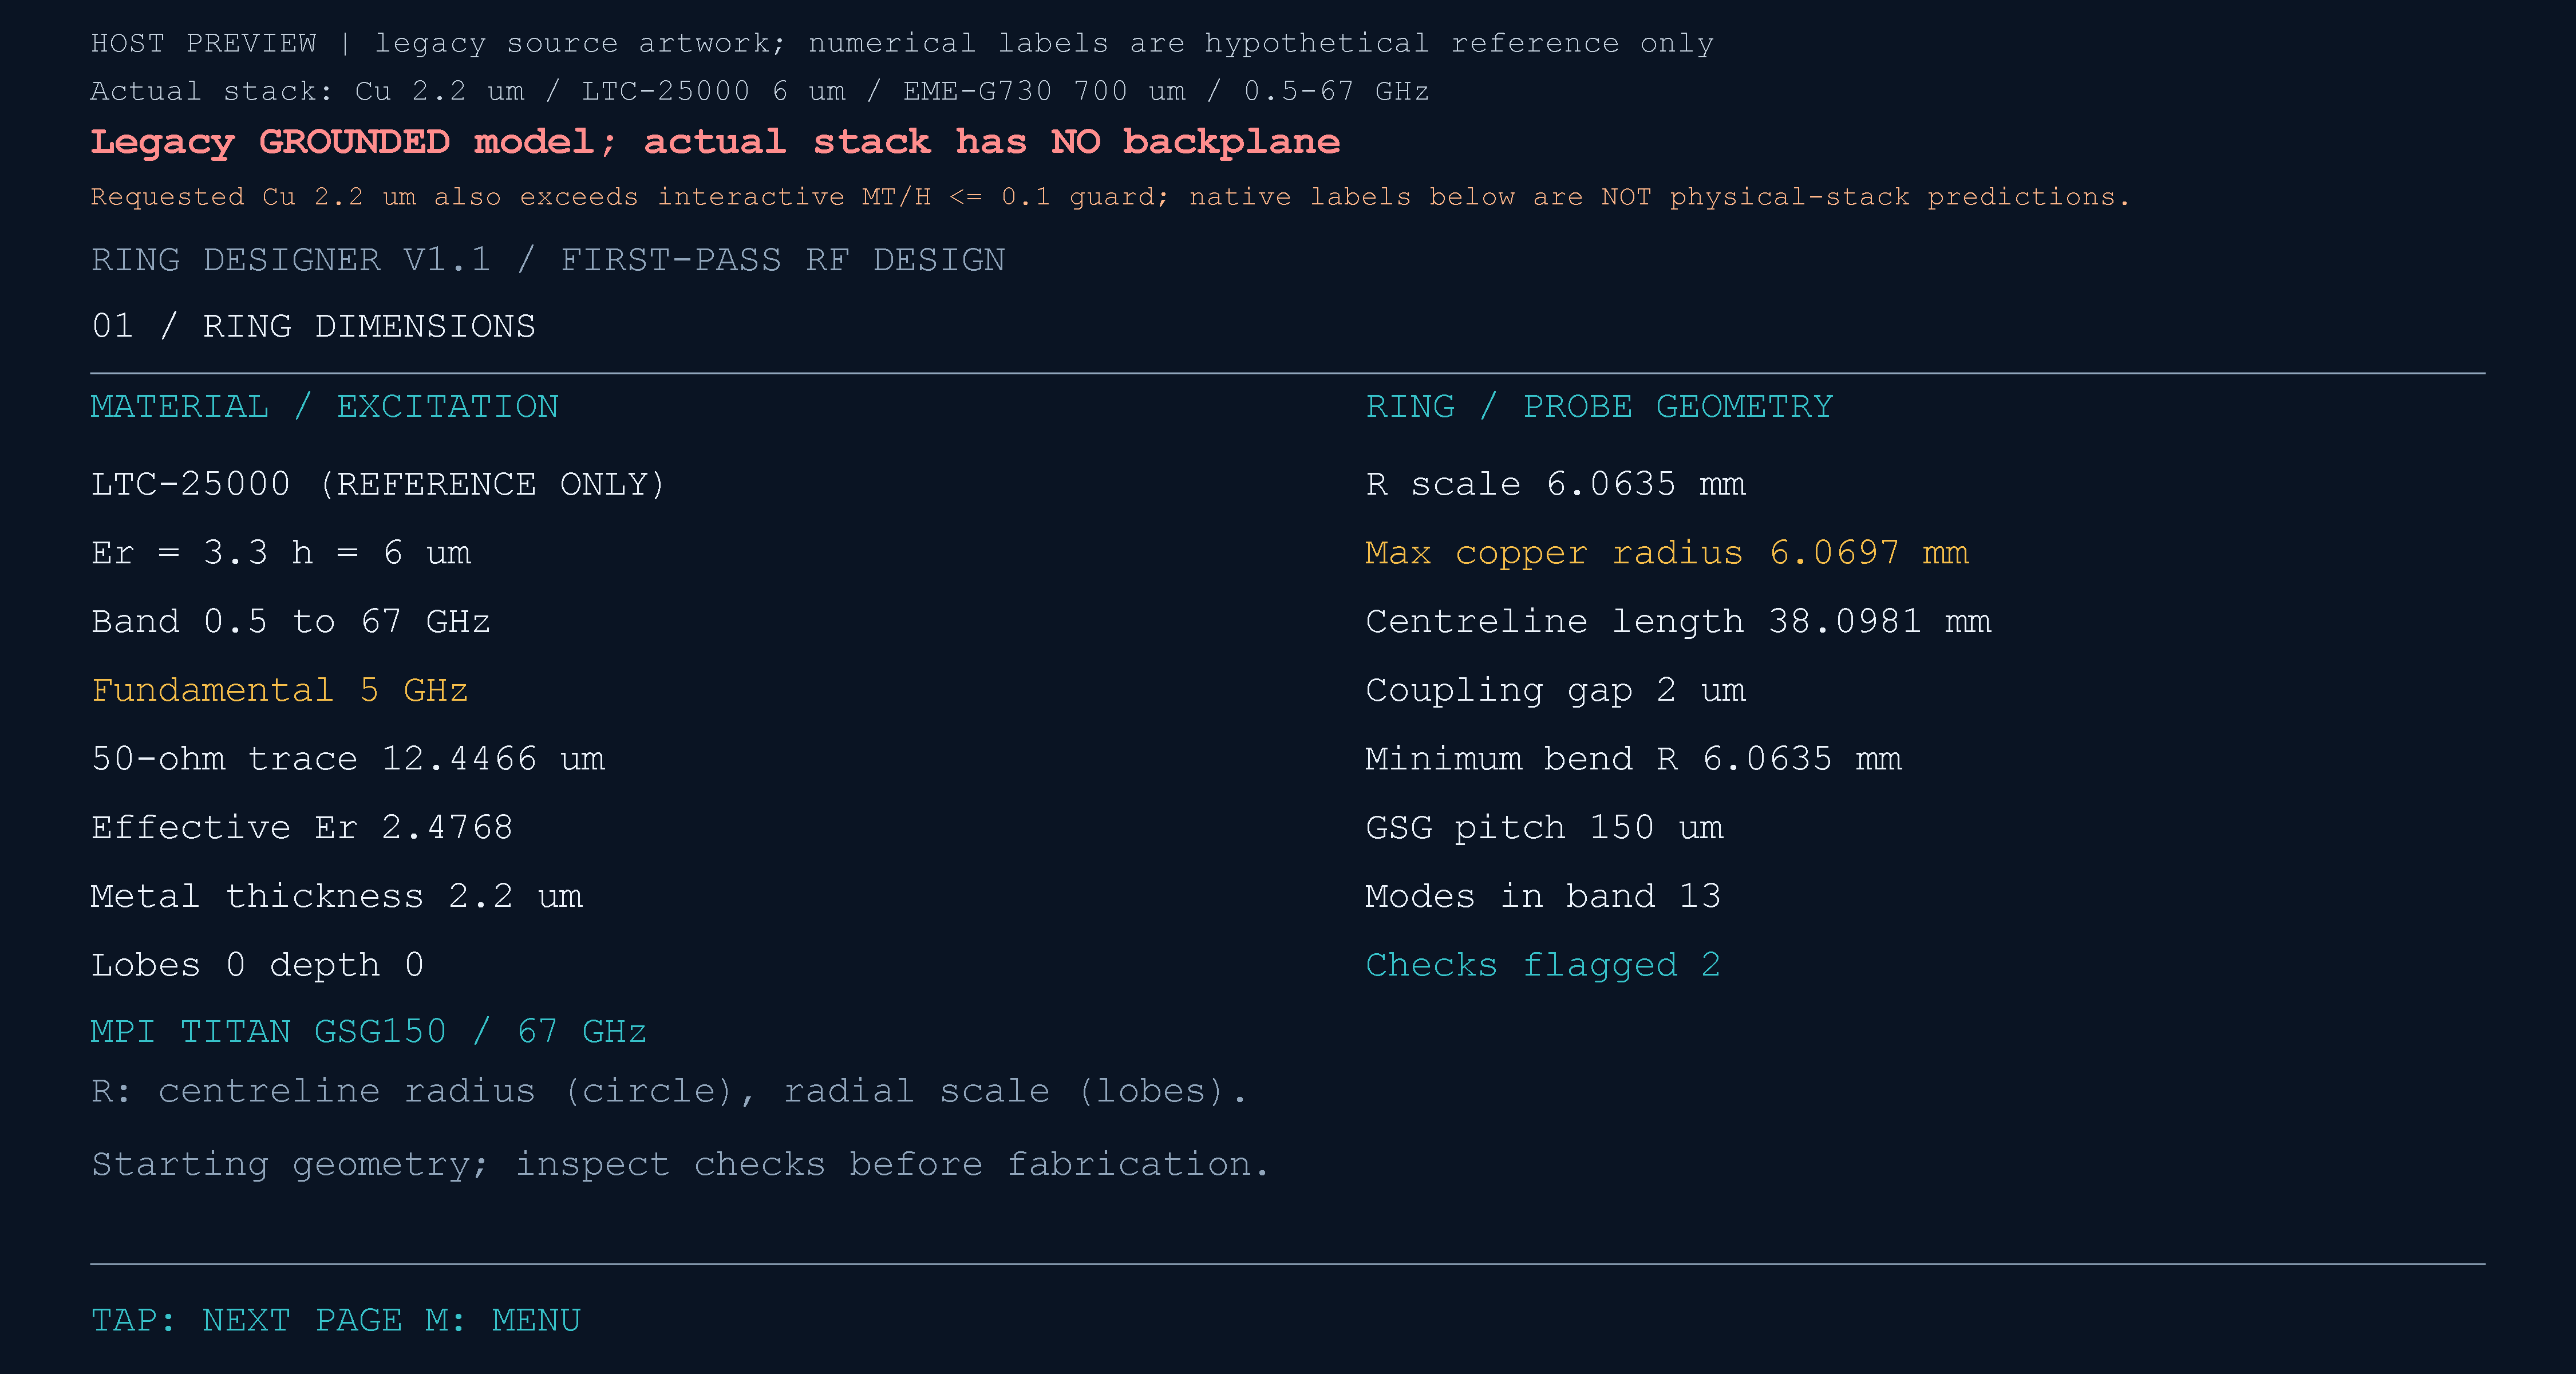
\includegraphics[width=.98\linewidth,height=.76\textheight,keepaspectratio]{assets/resonator2-dimensions.png}\end{center}
{\small The source reports a hypothetical 50 ohm trace of 12.4466 \ensuremath{\mu\mathrm{m}} and a ring radius of 6.0635 mm for an illustrative 5 GHz fundamental. Neither dimension is a synthesized CPW design for the actual mold stack.}
\end{landscape}

\clearpage\begin{landscape}
\pageTitle{Circular ring and west/east access}{RESONATOR2 / legacy grounded-model evaluation / no physical-stack electrical prediction}
\begin{center}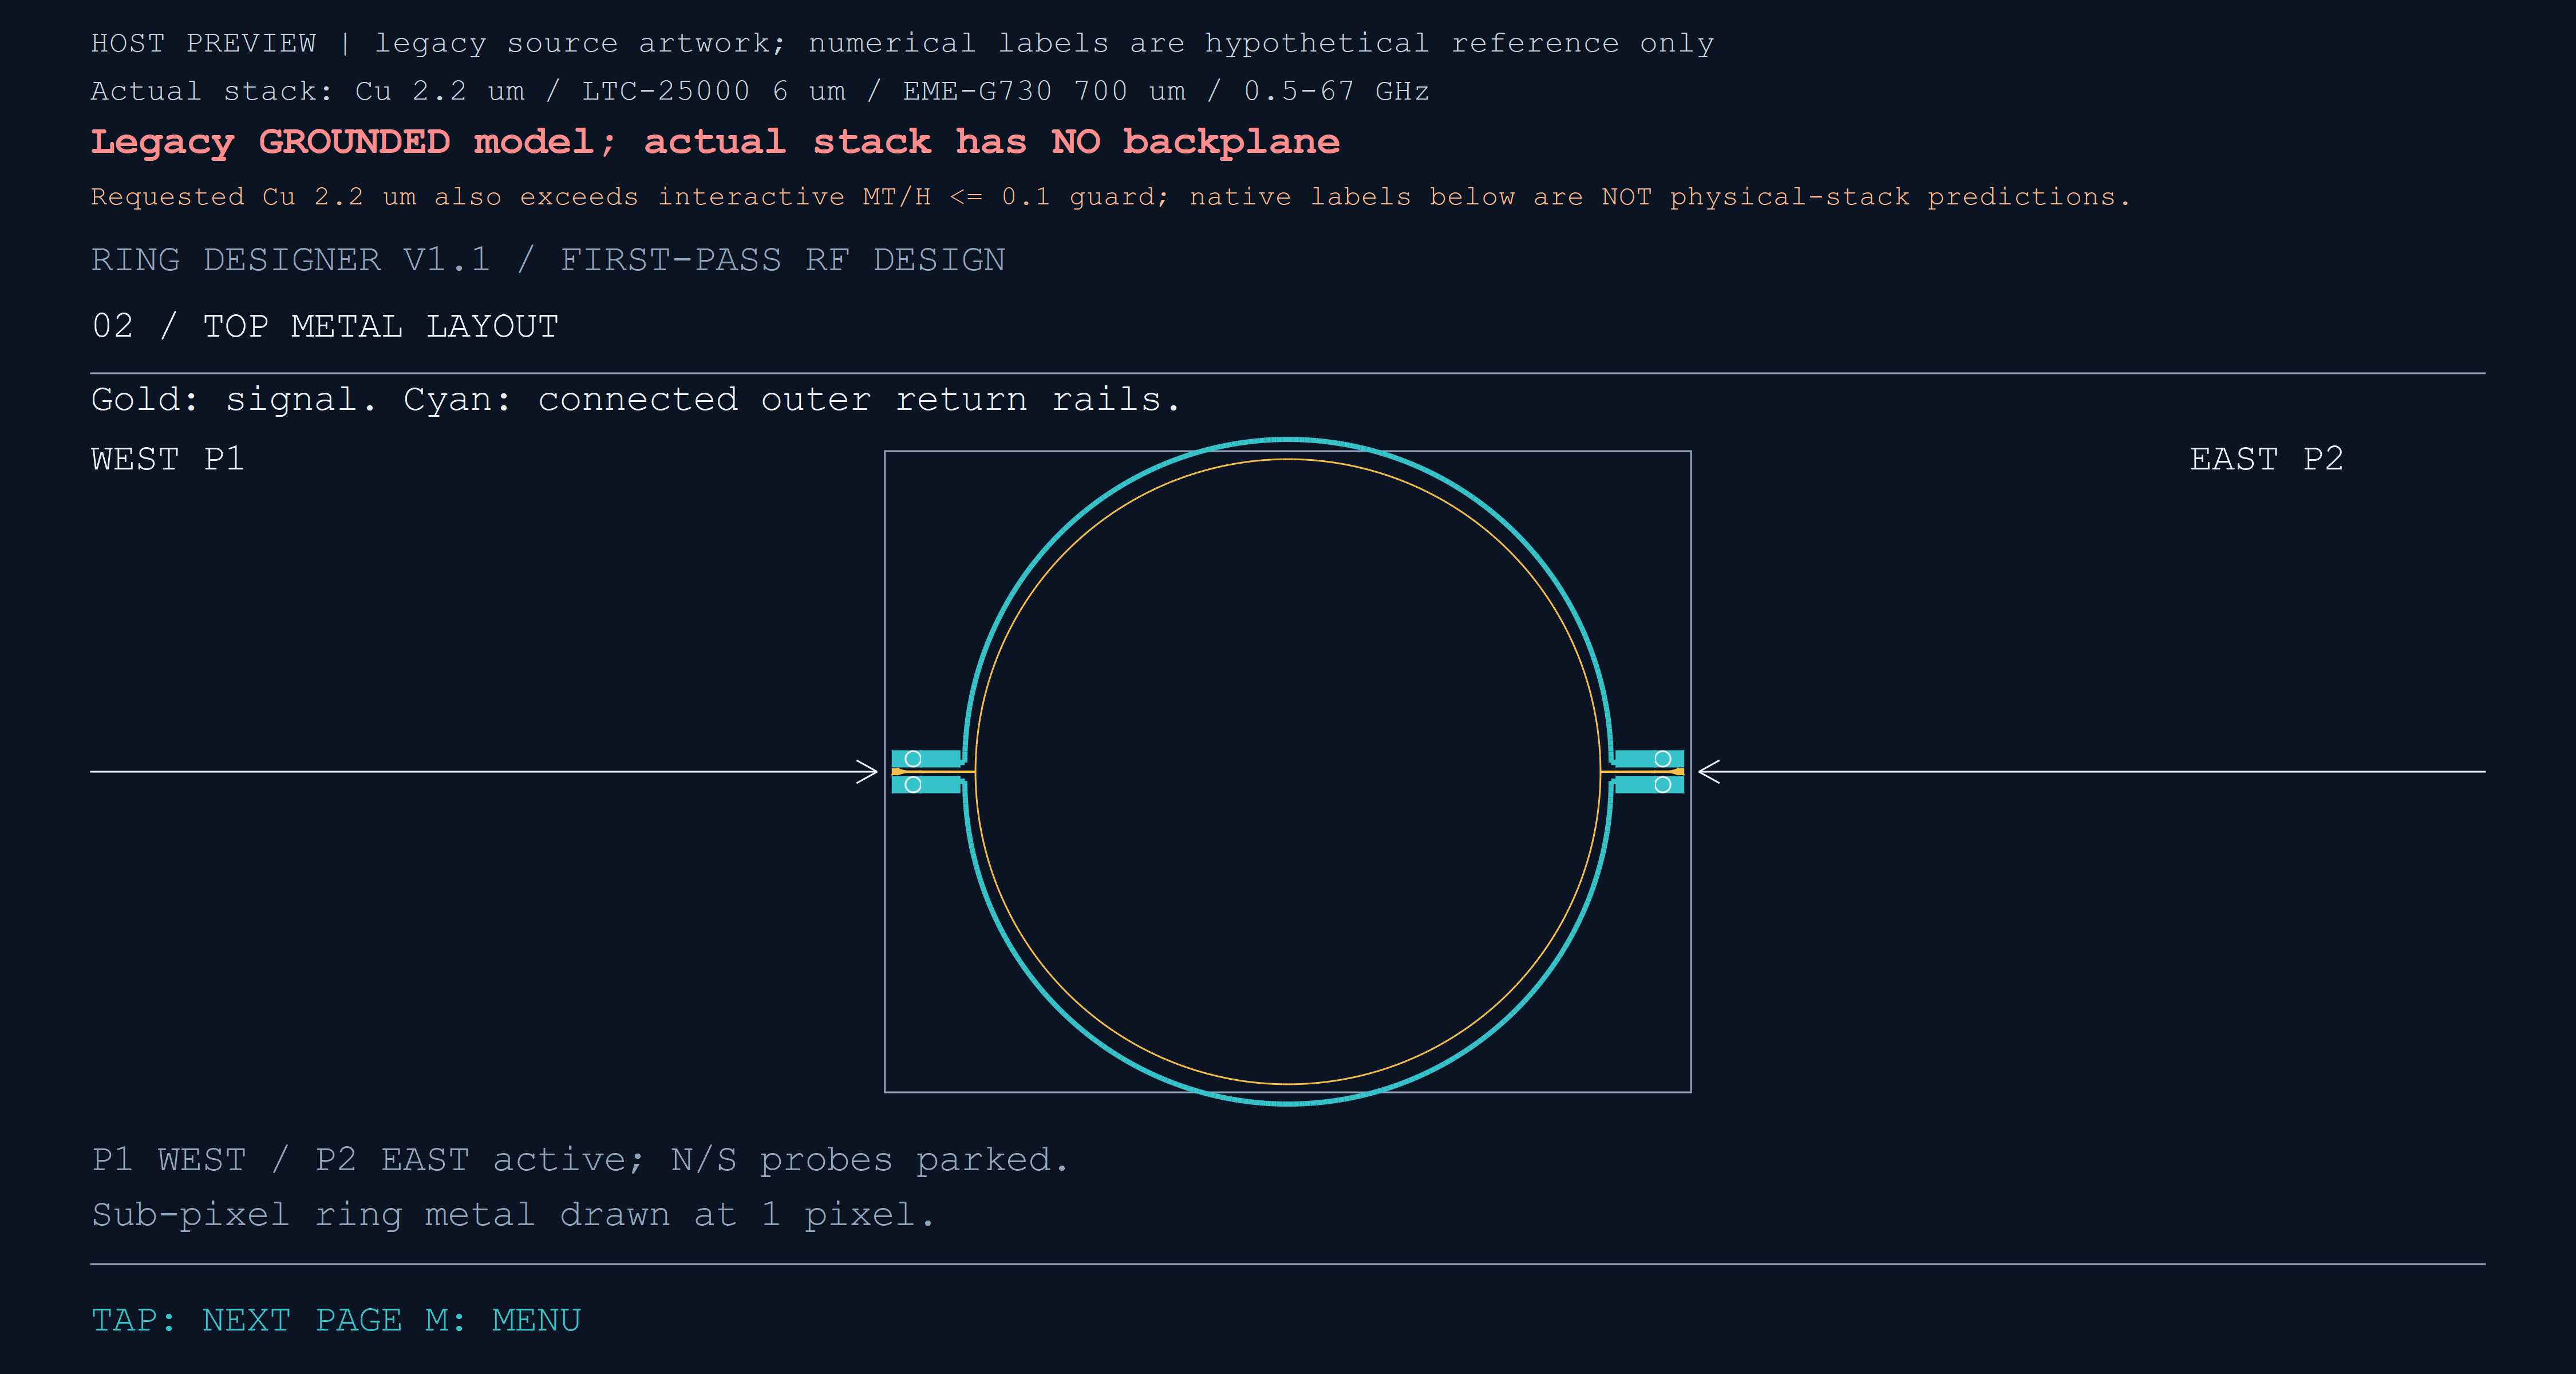
\includegraphics[width=.98\linewidth,height=.76\textheight,keepaspectratio]{assets/resonator2-circle.png}\end{center}
{\small Connected outer half-ring ground rails follow the signal and join both launch banks. No floating inner ground island is drawn. Rail and slot dimensions and feed-to-ring coupling still require an ungrounded multilayer model; the legacy numerical model assumes a continuous backplane.}
\end{landscape}

\clearpage\begin{landscape}
\pageTitle{GSG launch detail}{RESONATOR2 / legacy grounded-model evaluation / no physical-stack electrical prediction}
\begin{center}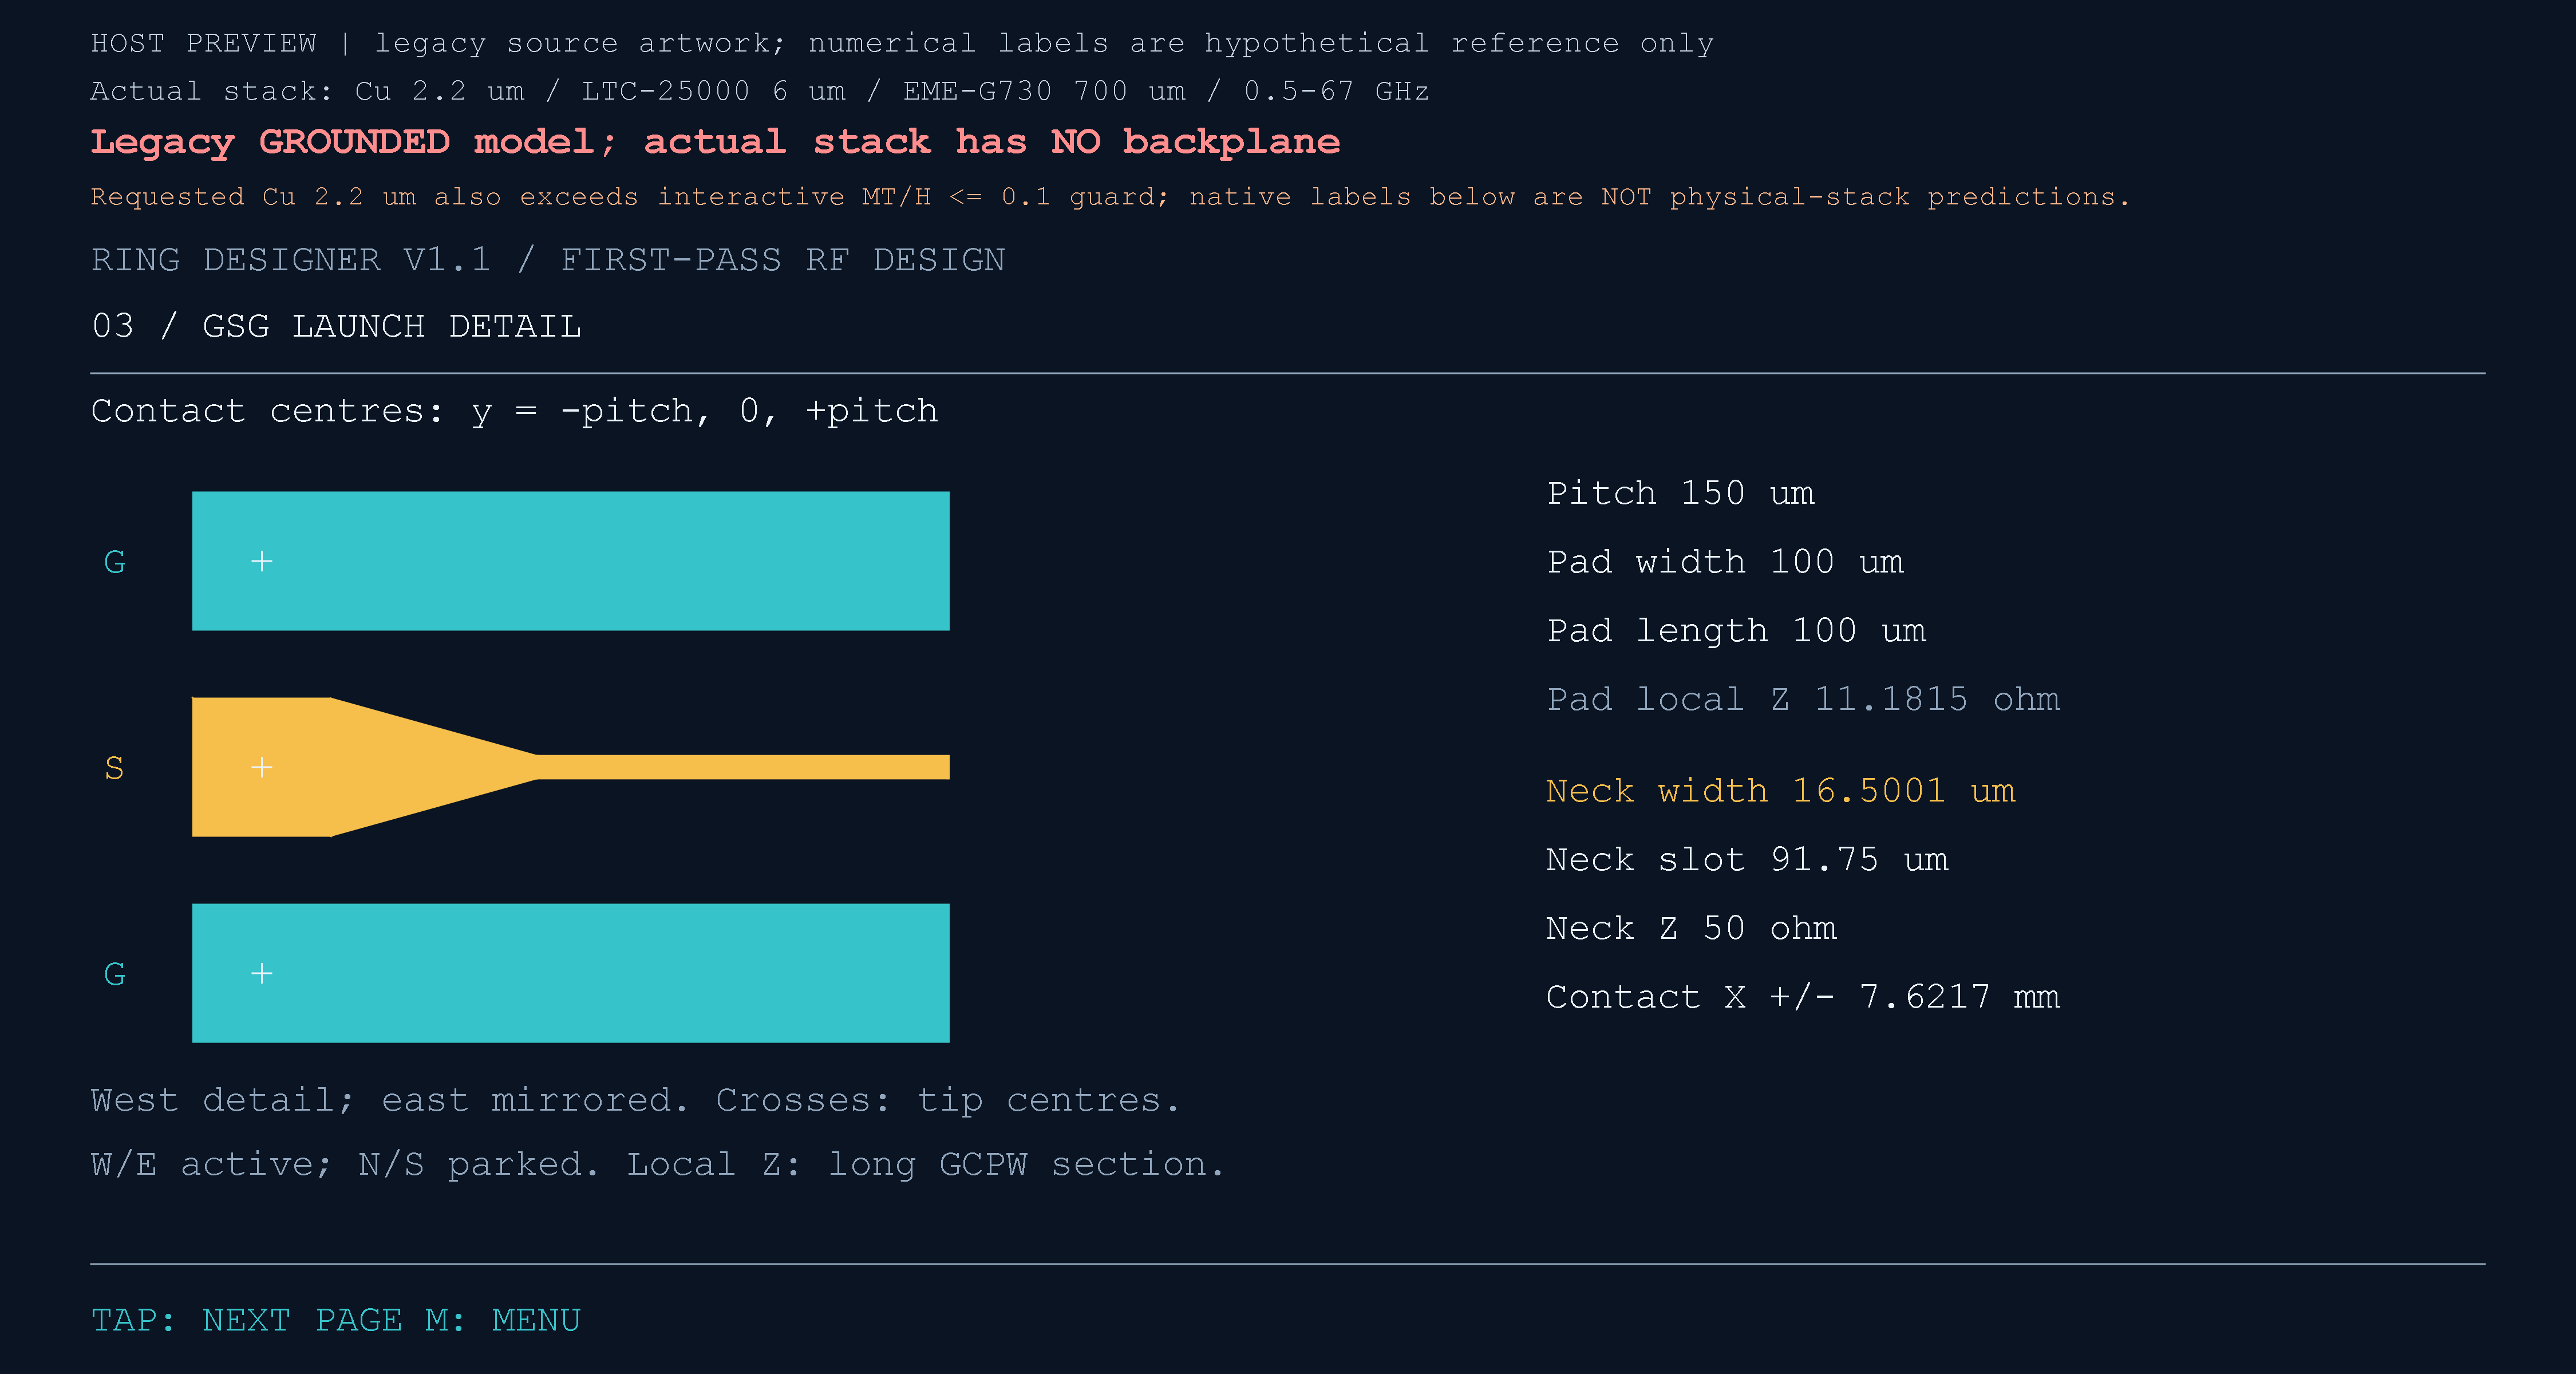
\includegraphics[width=.98\linewidth,height=.76\textheight,keepaspectratio]{assets/resonator2-gsg-launch.png}\end{center}
{\small The 150 \ensuremath{\mu\mathrm{m}} contact pitch is retained. The source launch uses a grounded-CPW approximation of zero metal thickness; its neck and pad impedance labels do not describe this ungrounded stack. The 2.2 \ensuremath{\mu\mathrm{m}} metal thickness must be included in a replacement launch model.}
\end{landscape}

\clearpage\begin{landscape}
\pageTitle{Nominal resonance-mode page}{RESONATOR2 / legacy grounded-model evaluation / no physical-stack electrical prediction}
\begin{center}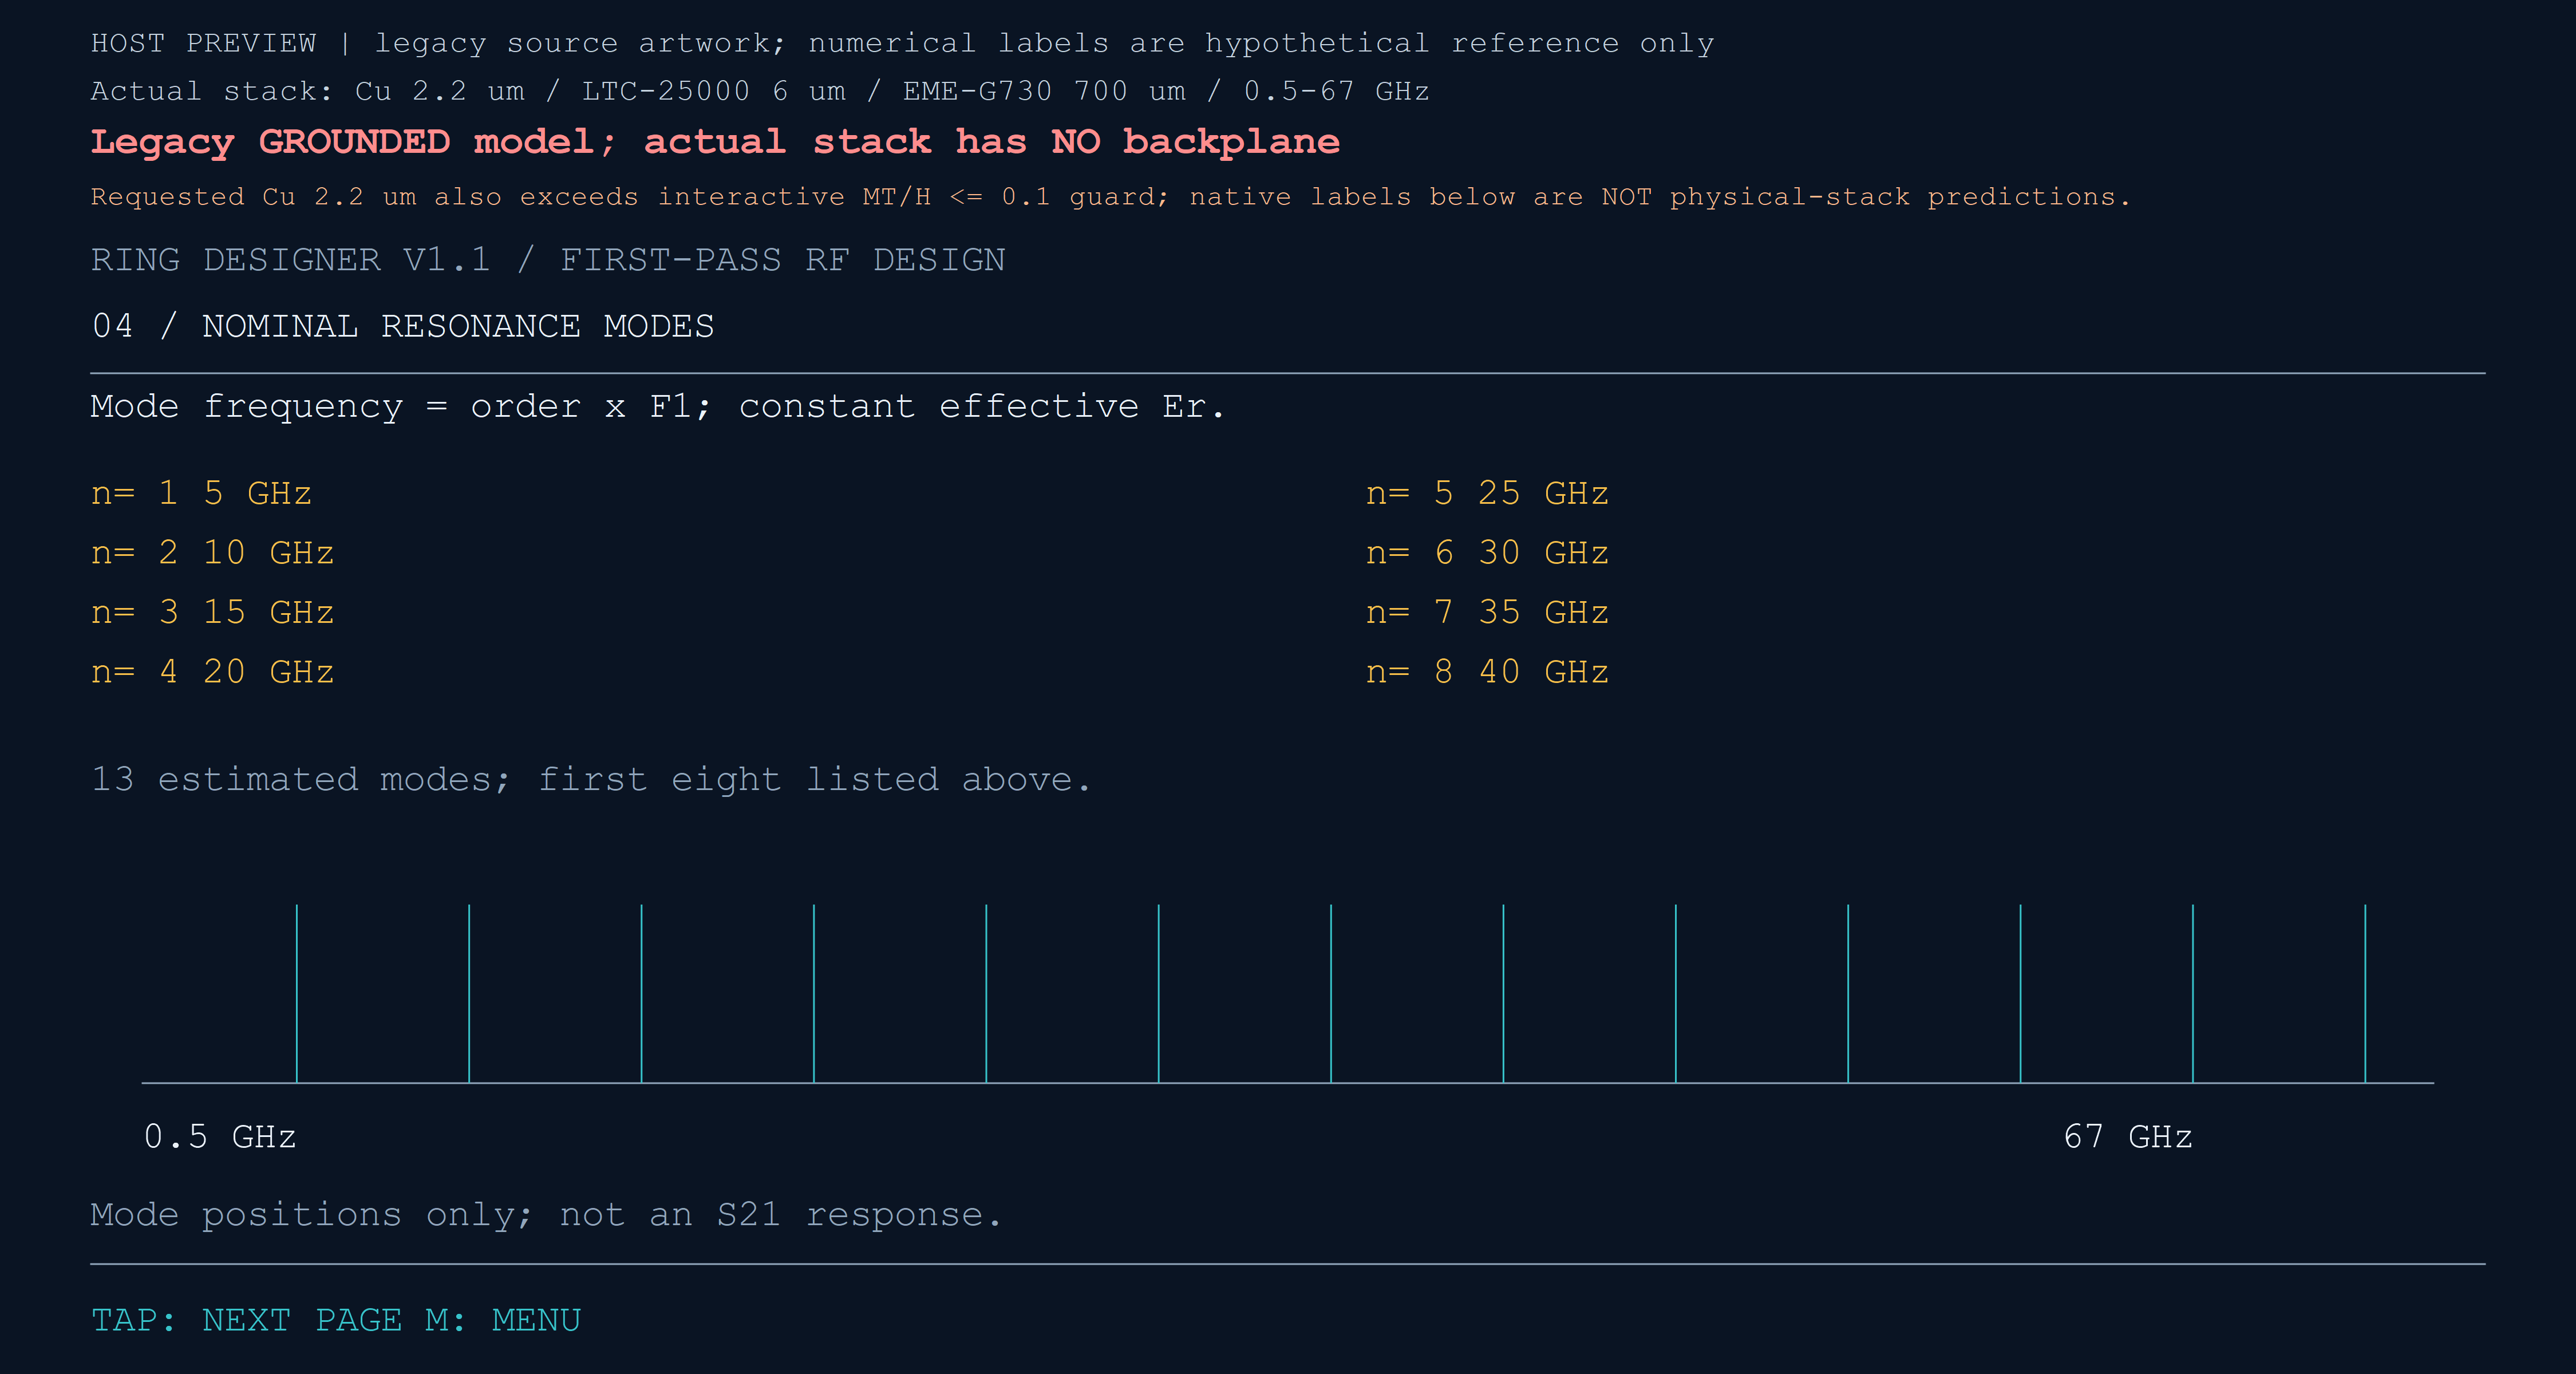
\includegraphics[width=.98\linewidth,height=.76\textheight,keepaspectratio]{assets/resonator2-modes.png}\end{center}
{\small A 5 GHz illustrative fundamental produces 13 nominal reference modes at 5,10,...,65 GHz. These are unloaded length-model positions, not measured resonances, not actual-stack predictions, and not an S21 passband.}
\end{landscape}

\clearpage\begin{landscape}
\pageTitle{Native model checks}{RESONATOR2 / legacy grounded-model evaluation / no physical-stack electrical prediction}
\begin{center}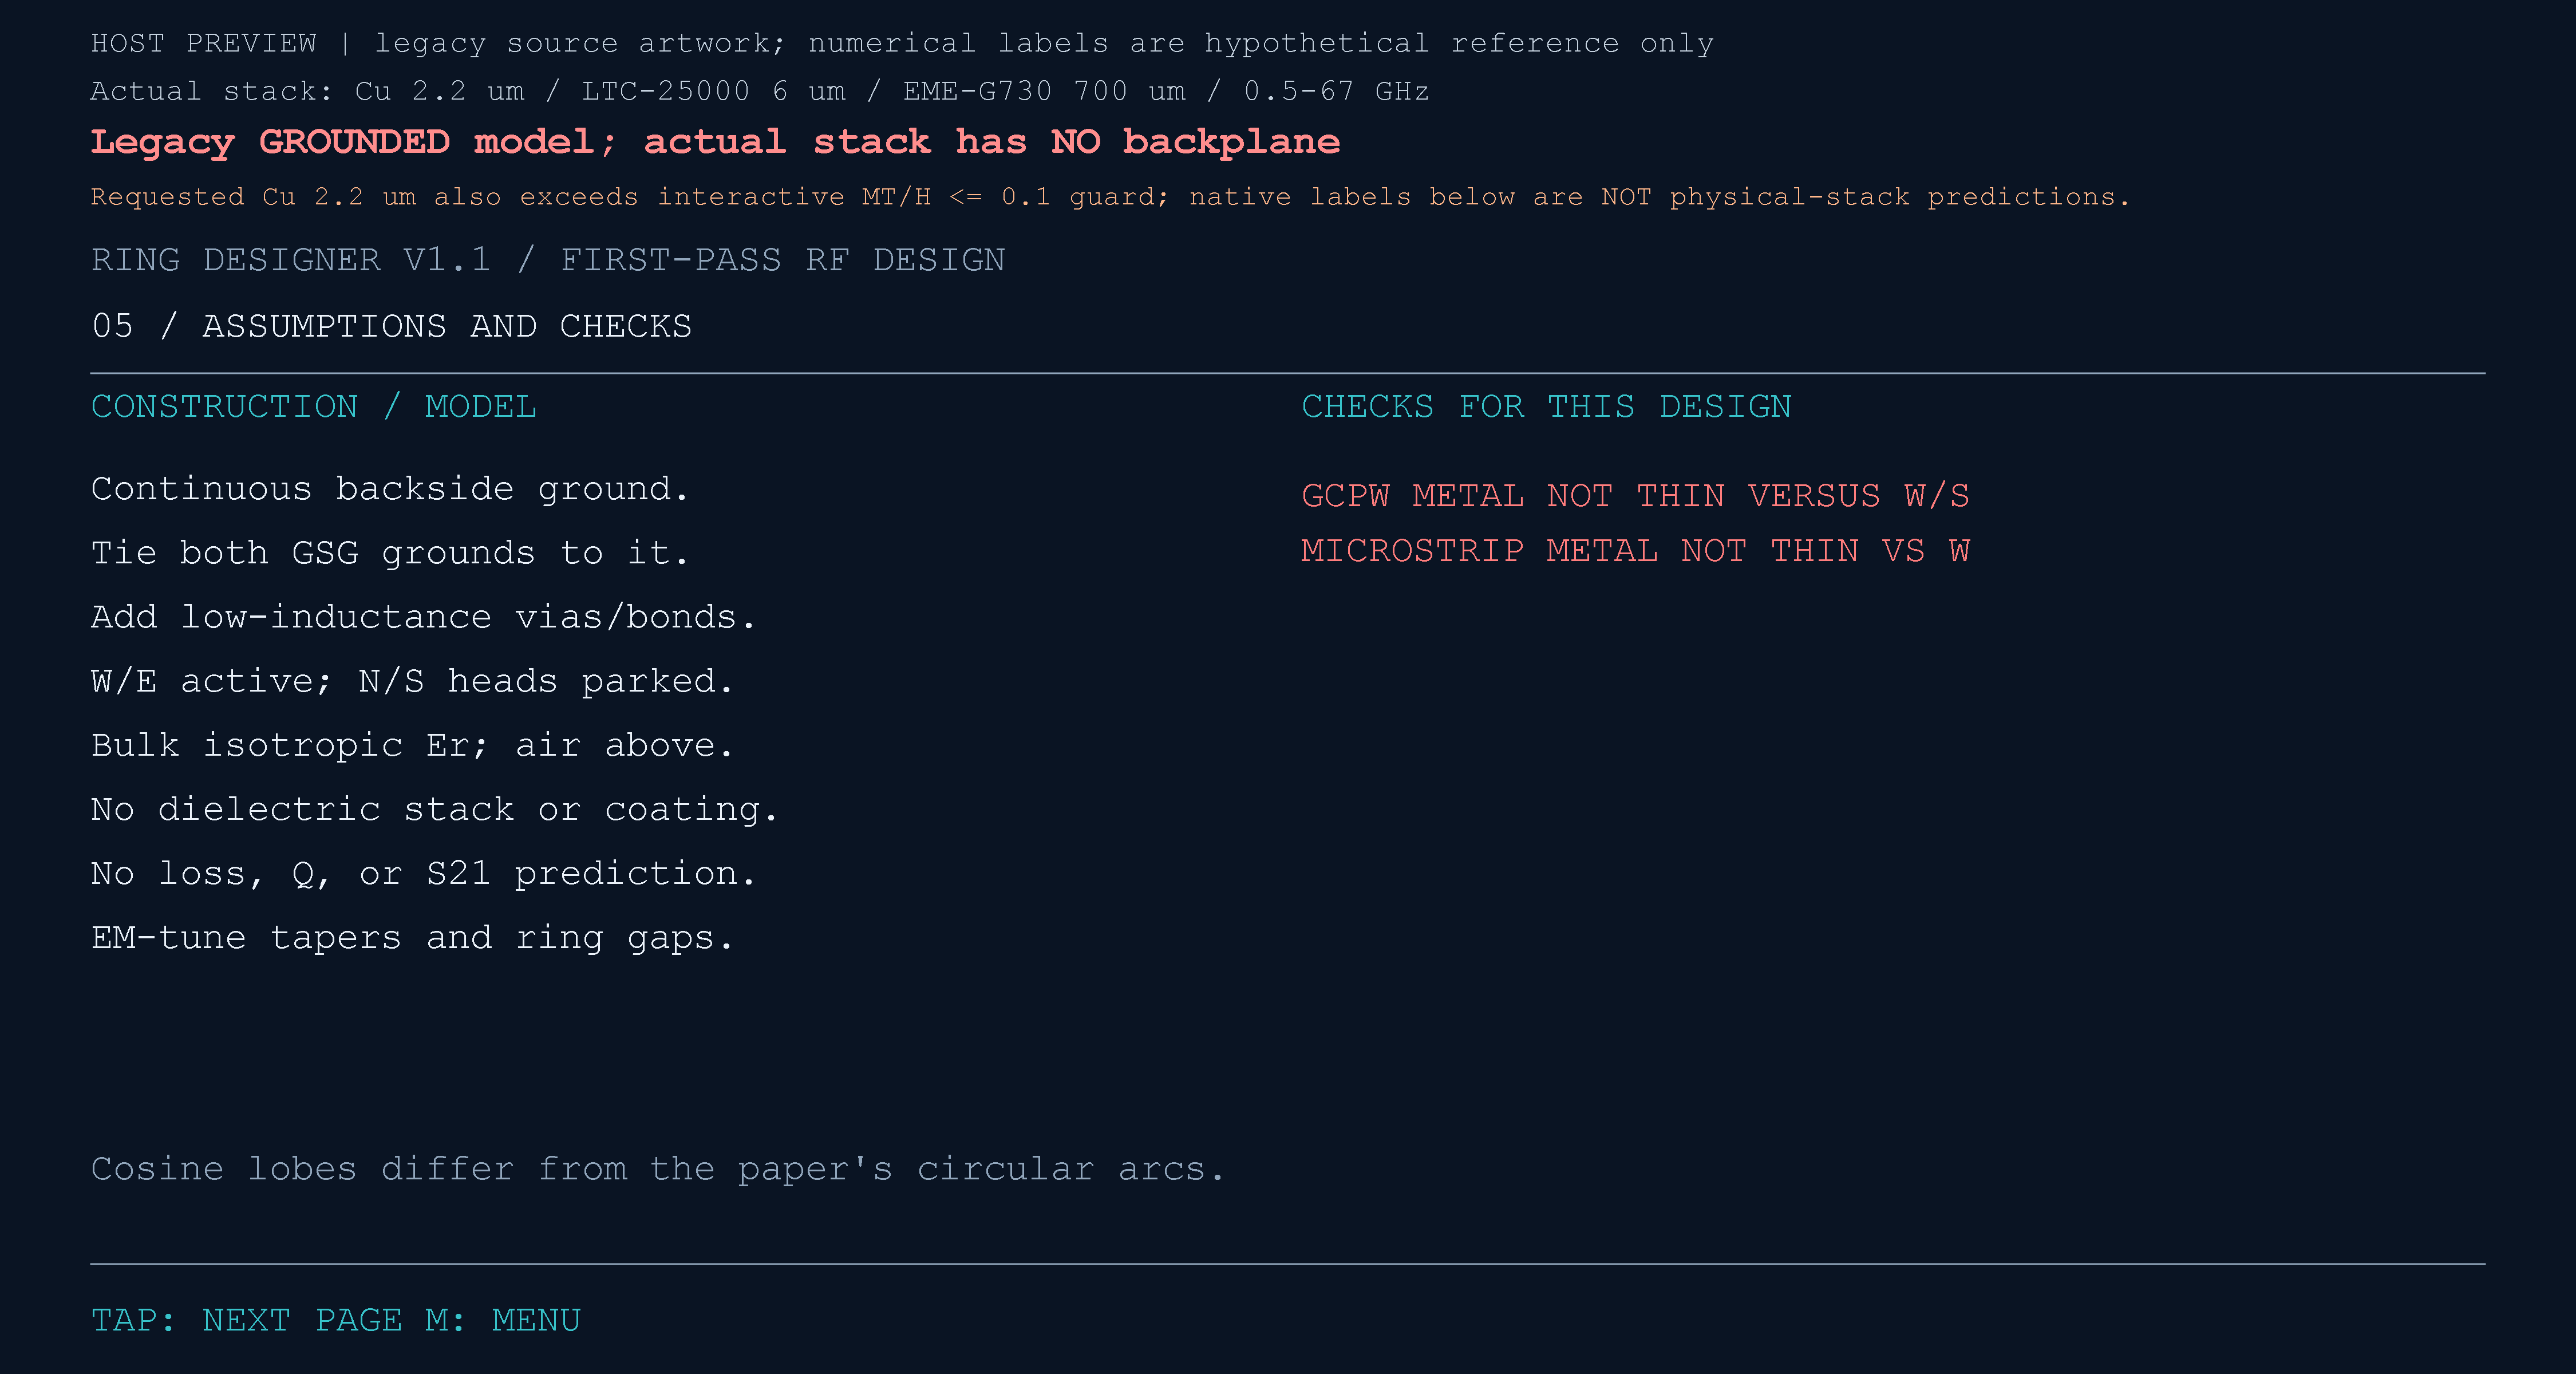
\includegraphics[width=.98\linewidth,height=.76\textheight,keepaspectratio]{assets/resonator2-checks.png}\end{center}
{\small At 6 \ensuremath{\mu\mathrm{m}} insulation, the source input guard permits at most 0.6 \ensuremath{\mu\mathrm{m}} copper; requested copper is 2.2 \ensuremath{\mu\mathrm{m}}. These host previews evaluate the unchanged equations directly outside that interactive guard. The source also flags both microstrip and GCPW thin-metal conditions.}
\end{landscape}

\clearpage\begin{landscape}
\pageTitle{Six-lobe source variant}{RESONATOR2 / legacy grounded-model evaluation / no physical-stack electrical prediction}
\begin{center}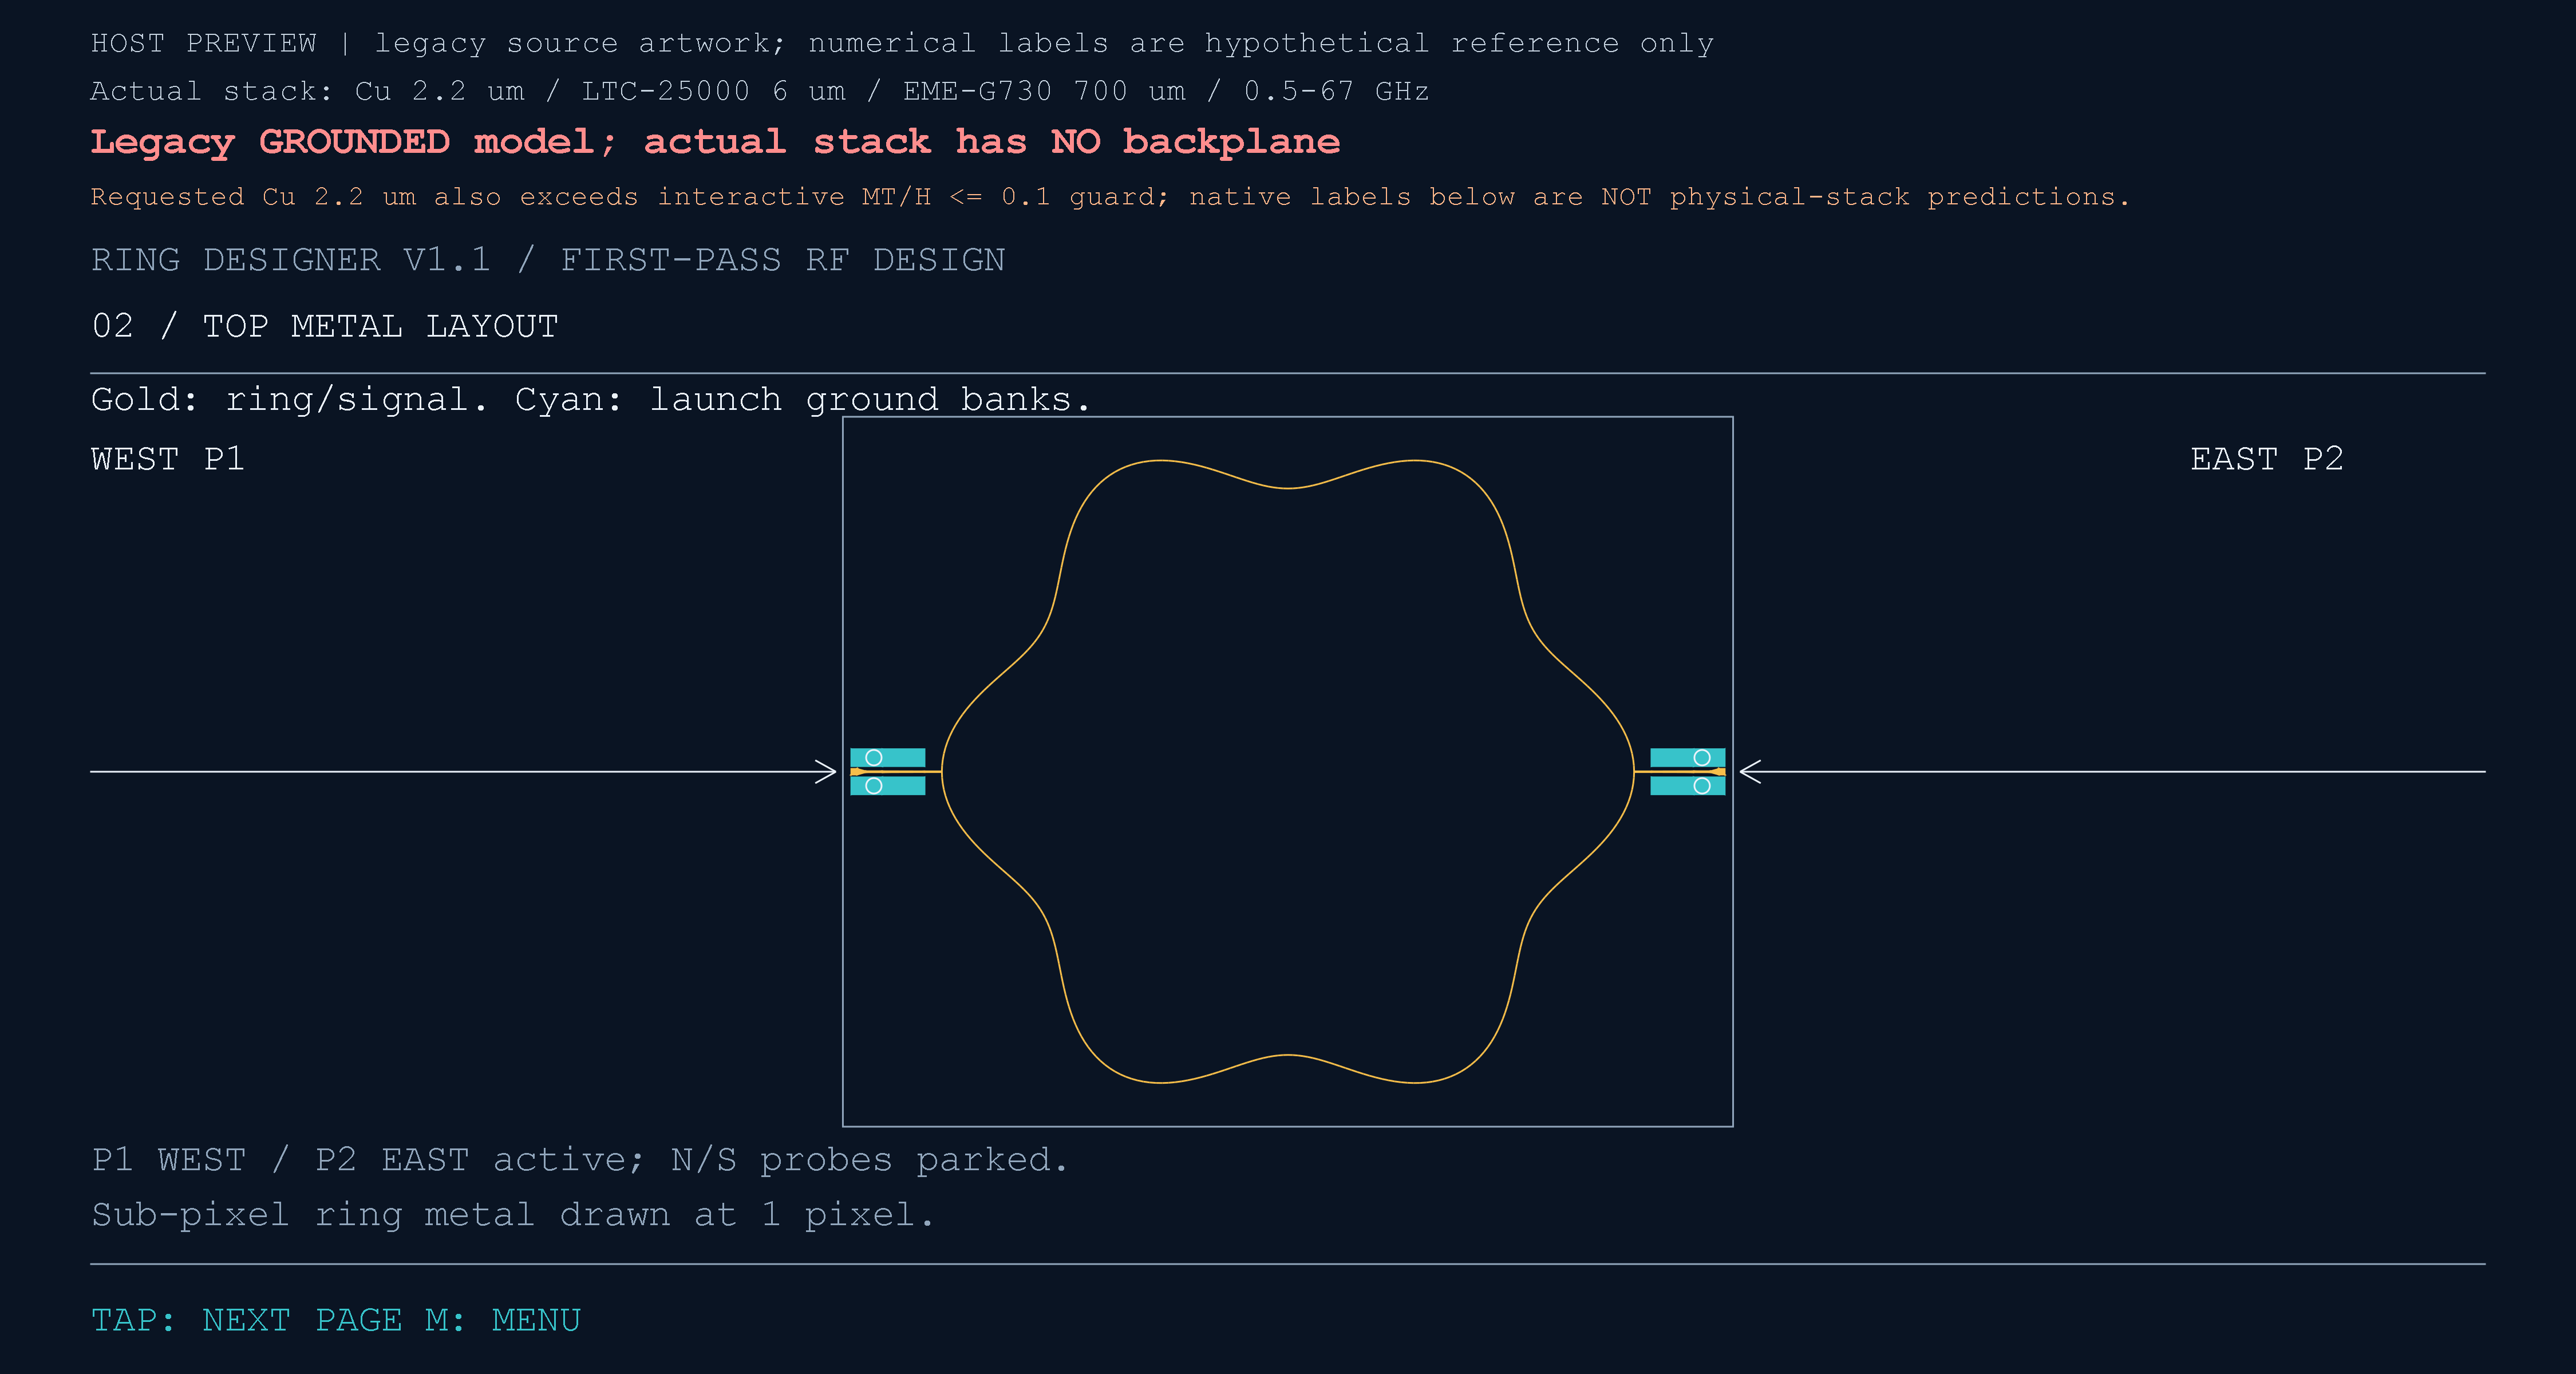
\includegraphics[width=.98\linewidth,height=.76\textheight,keepaspectratio]{assets/resonator2-six-lobes.png}\end{center}
{\small The extra variant uses six cosine lobes at 10 percent depth. It illustrates the source shape parameterization, not a validated alternative for the physical stack. It retains two west/east ports and parked north/south heads.}
\end{landscape}

\clearpage
\pageTitle{GDSII unit cells}{Eight ground-plane unit cells generated by CBM BASIC V2 scripts in the gds folder}
\subhead{What the scripts produce}
Each cell has its own script, for example \texttt{gds\_zcoupon.bas}, that asks for the stack parameters, synthesizes the 50 $\Omega$ width with the same Hammerstad--Jensen routine the report uses, and writes a binary GDSII stream \texttt{NAME.GDS}. The library name is RFTEST, the structure name equals the file name, and the database unit is 1 nm with a 1 $\mu$m user unit. Port labels sit on the signal pad of each G--S--G landing at 150 $\mu$m pitch.
\subhead{Ground plane}
At your request every cell carries a continuous ground plane on layer 1, directly beneath the 6 \ensuremath{\mu\mathrm{m}} polyimide. That is the condition the legacy models assume, so the reference numbers and expected data in this report apply to these cells directly, within the limits of the illustrative $\varepsilon_r$ and $\tan\delta$. The as-supplied stack has no plane. Dropping layer 1 and keeping the M1 ground rails gives the plane-less coplanar variant, for which the model changes listed with each structure are required. M1 ground rails follow each signal trace on both sides, and V0 via fences tie them to the plane.
\subhead{Layer map}
\par\noindent\begin{tabular}{@{}rlp{.72\linewidth}@{}}\toprule
Layer & Name & Use\\\midrule
1 & GND & continuous ground plane, one polygon over the whole cell plus a 150 $\mu$m margin\\
2 & V0 & vias from M1 down to the plane (ground fences, ground islands)\\
3 & M1 & first metal: signal lines, pads, ground rails\\
4 & V1 & vias between M1 and M2\\
5 & M2 & second metal: pads, feeds and jumpers where a layer change is drawn\\
7 & RES & resistor marker (not conductive)\\
10 & LABEL & port labels placed on the signal pads\\
11 & NOTE & annotation text\\\bottomrule
\end{tabular}\par

\subhead{Cells}
{\small \par\noindent\begin{tabular}{@{}llrrrp{.30\linewidth}@{}}\toprule
Cell & Script & Size (mm) & Vias & kB & Contents\\\midrule
ZCOUPON & gds\_zcoupon.bas & 6.20 $\times$ 2.54 & 384 & 38.8 & three 5 mm lines at 0.9, 1.0 and 1.1 times the 50 ohm width\\
RDLLOSS & gds\_rdlloss.bas & 3.59 $\times$ 2.54 & 216 & 23.0 & three lines of 2.000, 2.196 and 2.392 mm\\
STUBTEST & gds\_stubtest.bas & 1.80 $\times$ 10.12 & 268 & 29.4 & three-port through lines with north-facing P3 at each stub end\\
TRLSET & gds\_trlset.bas & 30.20 $\times$ 5.54 & 1056 & 104.3 & thru, four lines of 28.996 to 1.711 mm, and an open reflect\\
RFLEAK & gds\_rfleak.bas & 5.20 $\times$ 0.54 & 148 & 15.9 & M2 pads, 4 mm M1 line, V1 transitions with ground vias\\
VIAMATCH & gds\_viamatch.bas & 2.30 $\times$ 2.54 & 120 & 14.4 & bare stud, matched stud with L-C network, back-to-back studs\\
RDXTALK & gds\_rdxtalk.bas & 6.46 $\times$ 5.73 & 474 & 50.4 & four-port crosstalk coupons at 10, 20 and 40 \ensuremath{\mu\mathrm{m}} gap\\
RESONATOR2 & gds\_resonator2.bas & 15.34 $\times$ 12.69 & 246 & 31.5 & ring resonator with 2 \ensuremath{\mu\mathrm{m}} coupling gaps and ground arcs\\\bottomrule
\end{tabular}\par
}
\subhead{Checks and generation}
\texttt{gds/verify\_gds.mjs} re-reads each stream and confirms the record structure and units, that polygons are closed and only the layers above appear, that one plane polygon extends at least 100 $\mu$m beyond all other geometry, and that vias join the intended layers. It also checks port labels: each sits on metal and off the plane net, and the ground pads at $\pm150\ \mu$m are tied to the plane. This report build runs the same checks and stops if any cell fails.
Generate the cells with \texttt{powershell -File gds/run\_gds.ps1}. The scripts call \texttt{SYSTEM}, so they need an SDL build of cbmbasic. The stream is first written as ASCII hex because text-mode file output turns each 0x0A byte into 0x0D 0x0A; the script then decodes it with \texttt{certutil} on Windows or \texttt{xxd} elsewhere. Two deliberate differences from the legacy programs: RFLEAK is drawn as a via-connected layer transition rather than an isolated plate, and the ring uses the synthesized microstrip width ($12.431\ \mu$m) instead of the grounded-CPW value ($12.447\ \mu$m).
\gdsfig{ZCOUPON}{ZCOUPON.GDS: three 5 mm lines at 0.9, 1.0 and 1.1 times the 50 ohm width.}
\gdsfig{RDLLOSS}{RDLLOSS.GDS: three lines of 2.000, 2.196 and 2.392 mm.}
\gdsfig{STUBTEST}{STUBTEST.GDS (rotated 90 degrees): three-port through lines with north-facing P3 at each stub end.}
\gdsfig{TRLSET}{TRLSET.GDS: thru, four lines of 28.996 to 1.711 mm, and an open reflect.}
\gdsfig{RFLEAK}{RFLEAK.GDS: M2 pads, 4 mm M1 line, V1 transitions with ground vias.}
\gdsfig{VIAMATCH}{VIAMATCH.GDS: bare stud, matched stud with L-C network, back-to-back studs.}
\gdsfig{RDXTALK}{RDXTALK.GDS: four-port crosstalk coupons at 10, 20 and 40 \ensuremath{\mu\mathrm{m}} gap.}
\gdsfig{RESONATOR2}{RESONATOR2.GDS: ring resonator with 2 \ensuremath{\mu\mathrm{m}} coupling gaps and ground arcs.}

\clearpage
\pageTitle{Mathematical utilities}{Source text previews complete the ten-program Hand BASIC inventory}
\begin{center}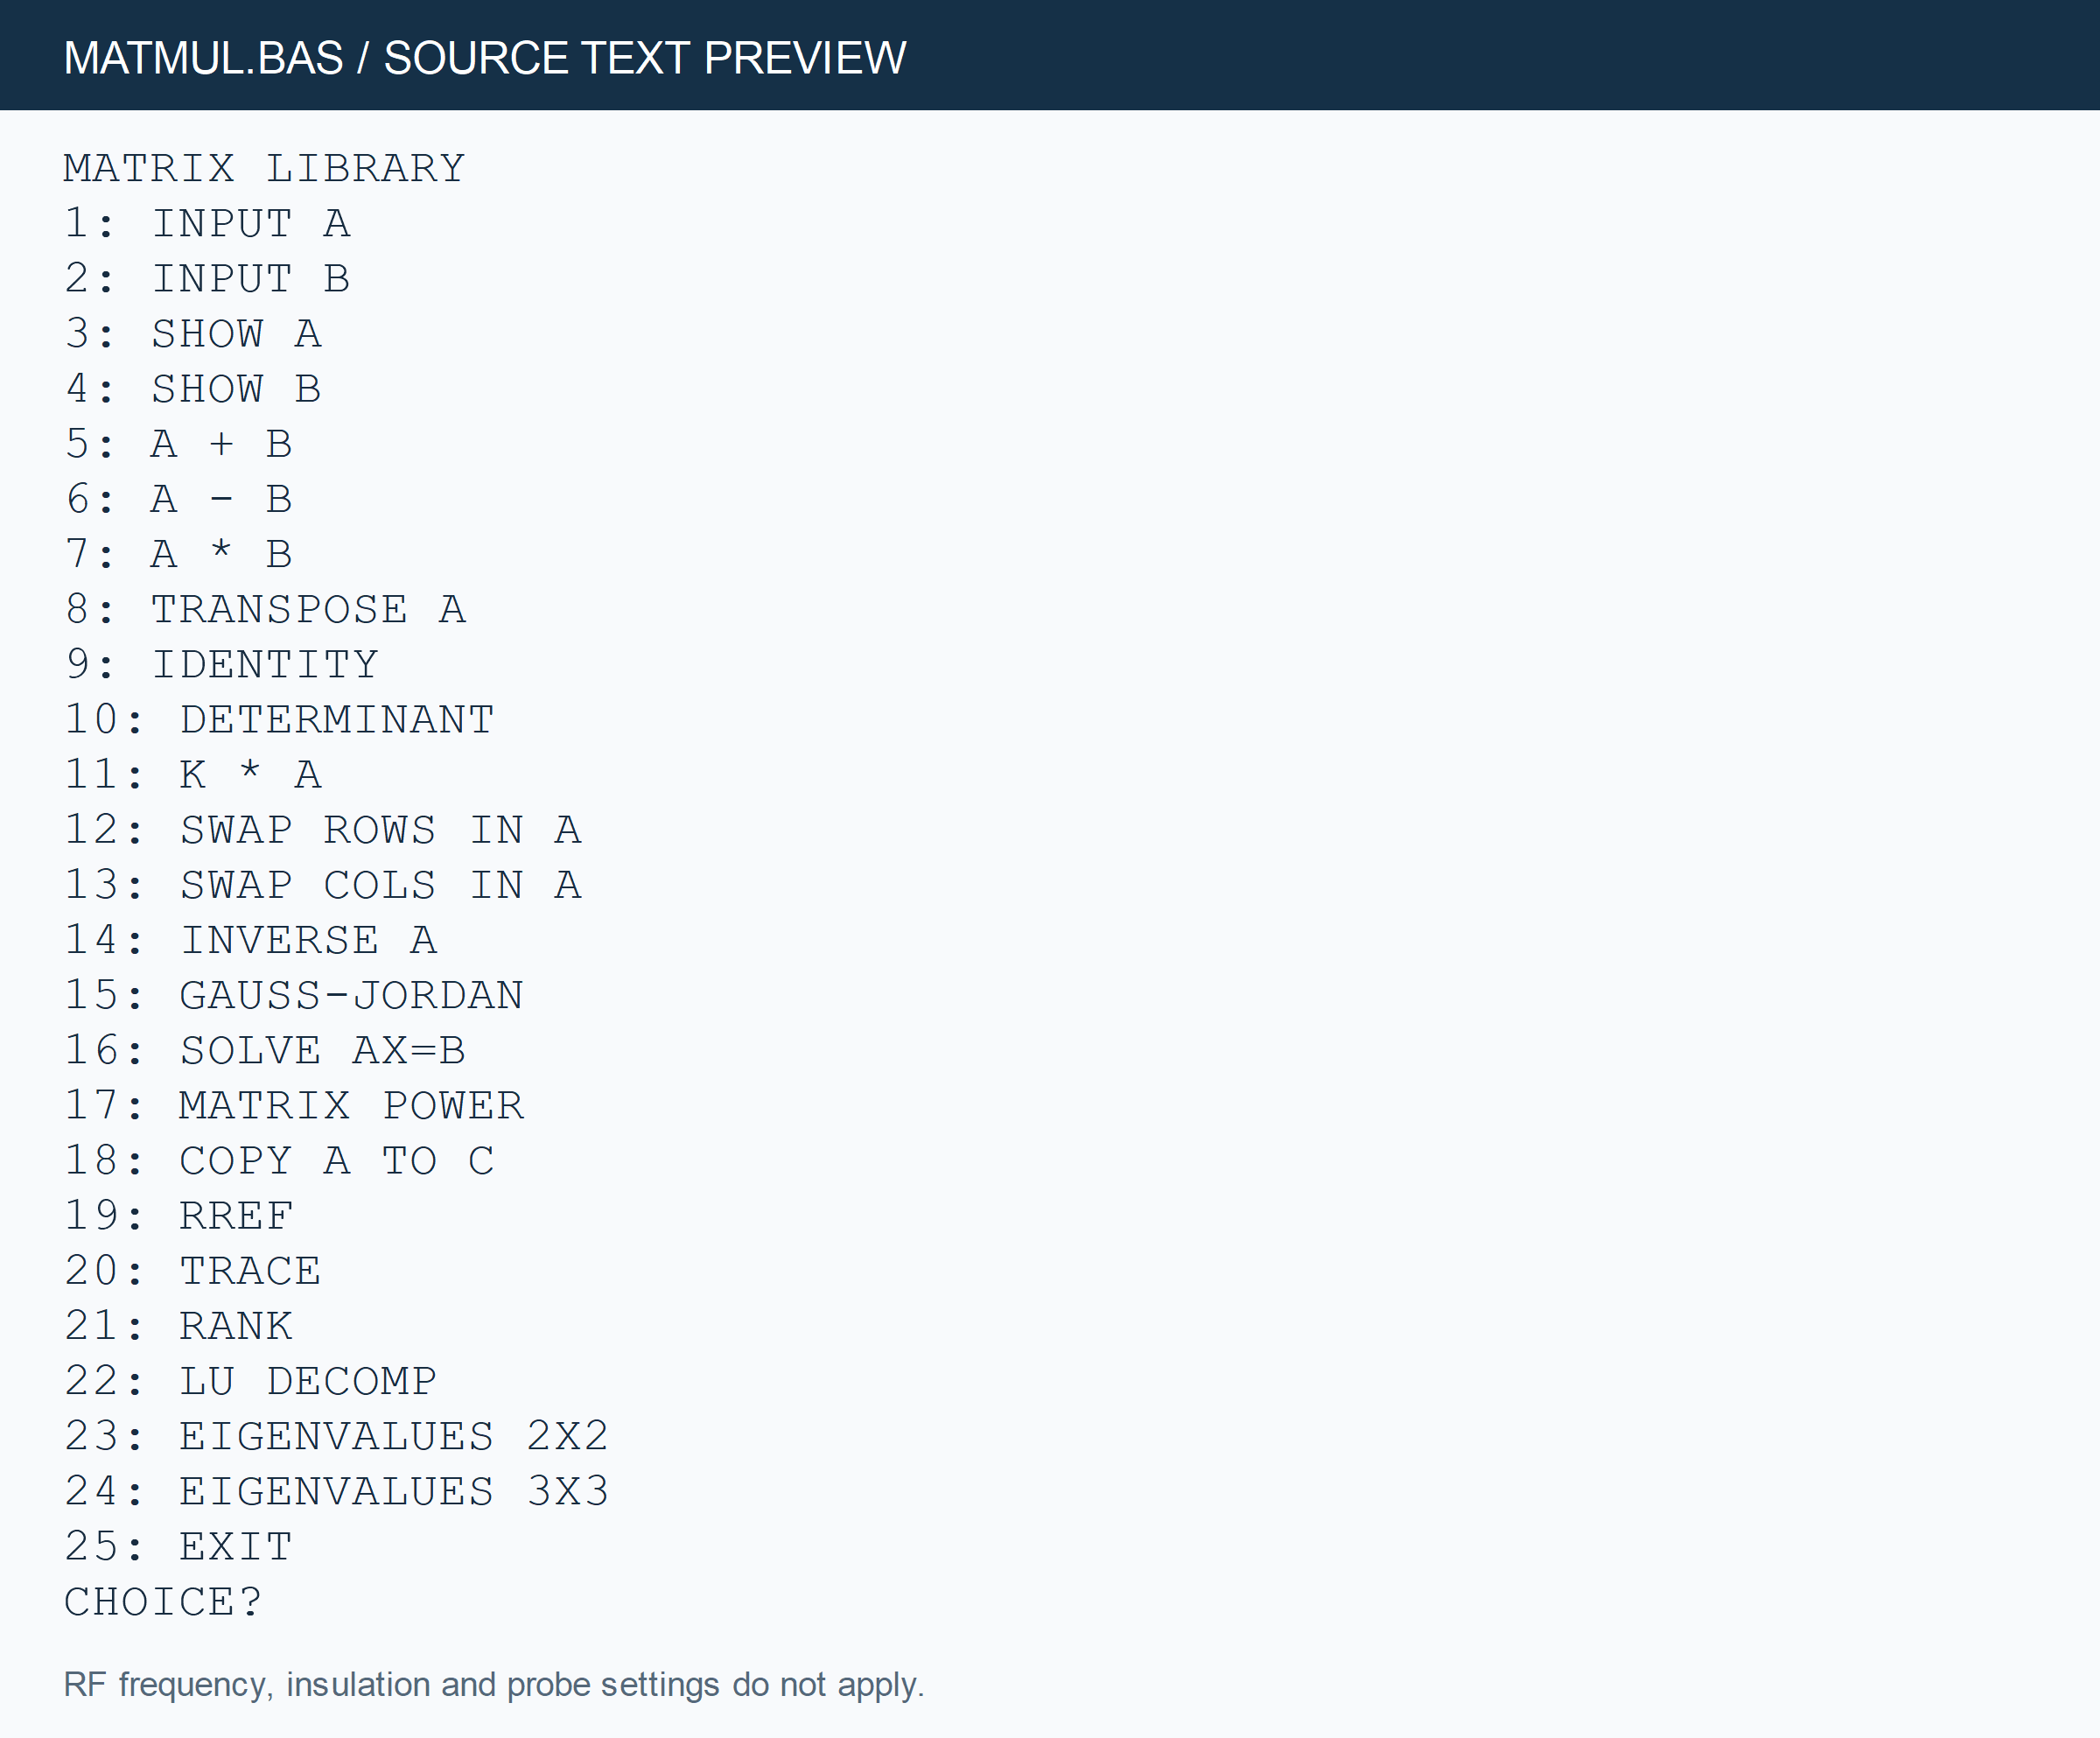
\includegraphics[width=.94\linewidth,height=.60\textheight,keepaspectratio]{assets/matmul.png}\end{center}
\begin{center}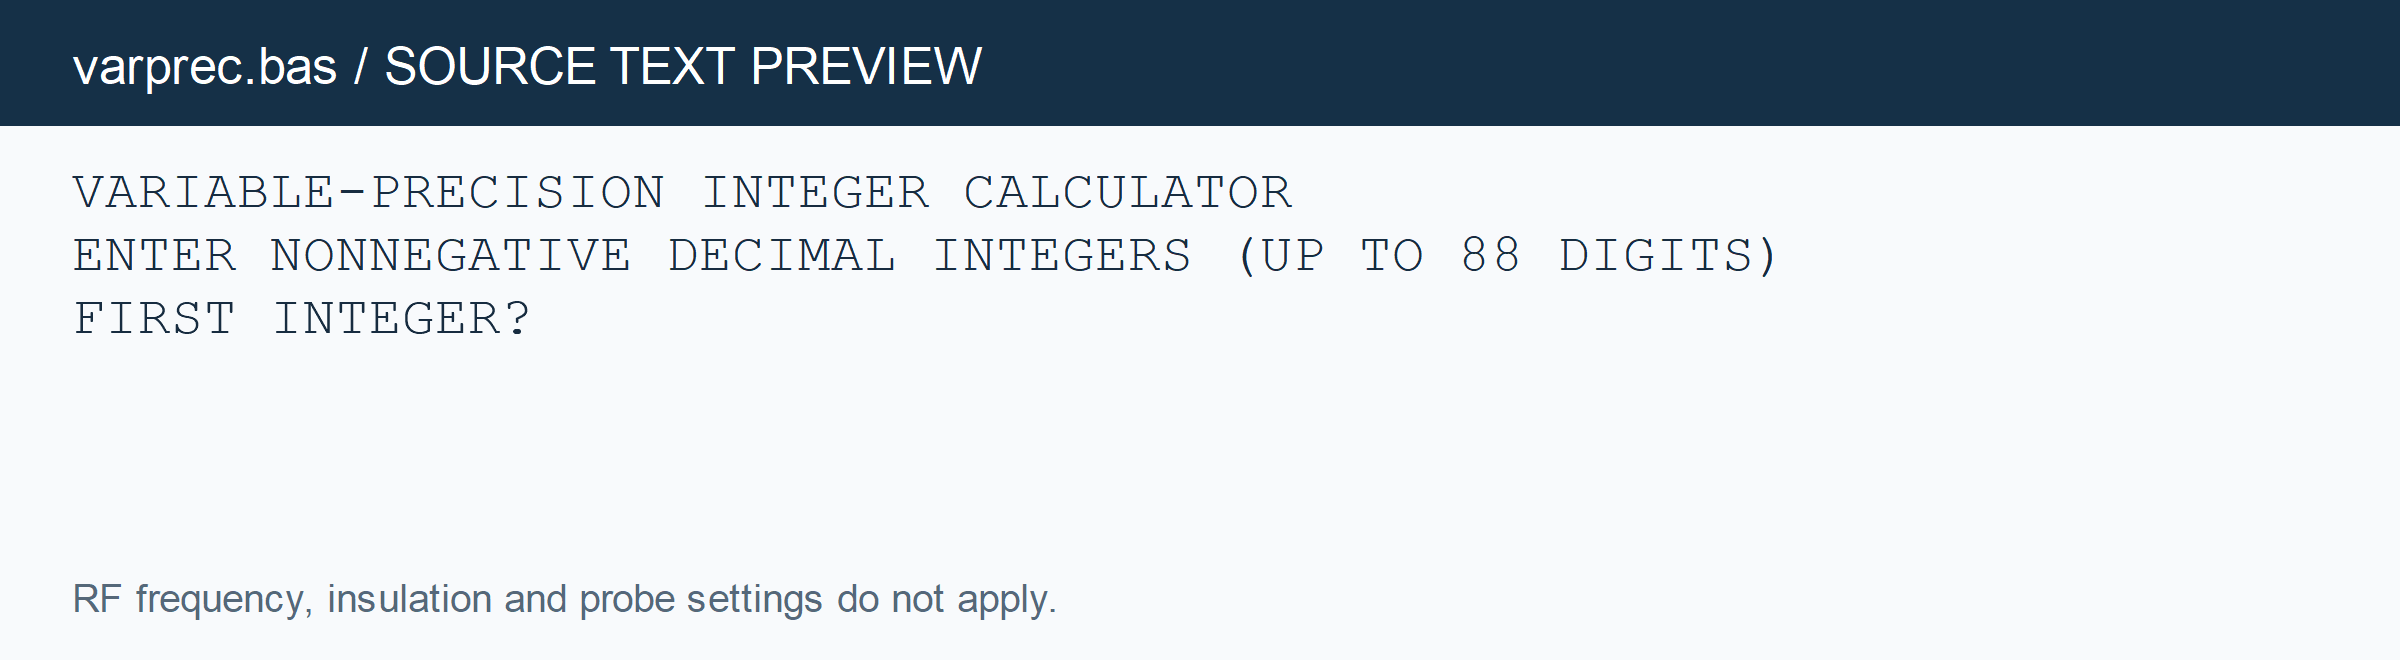
\includegraphics[width=.94\linewidth,height=.19\textheight,keepaspectratio]{assets/varprec.png}\end{center}
These two programs have no RF frequency, dielectric, copper or probe inputs. The previews extract the actual initial PRINT text and first INPUT prompt; menu actions and arithmetic are not executed by the preview generator.
\newpage
\pageTitle{Archived reference calculations}{Debugging the existing equations; excluded from actual-stack design claims}
\callout{\textbf{This archive does not solve the physical stack.} Microstrip widths and line responses assume a hypothetical continuous plane under the polyimide. Leakage capacitance and via matching use separate idealized plate and closed-return surrogates. The ungrounded multilayer structure is not solved. Agreement with source equations establishes reproducibility only. The GDSII unit cells do draw that continuous plane, so the reference curves describe them but not the as-supplied stack.}
The archive uses er=3.3, loss tangent=0.01, copper resistivity=17.2 nOhm m and RMS roughness=0.3 \ensuremath{\mu\mathrm{m}}. The last two values are retained source defaults; none is a measurement on this fabrication. Source equations were translated independently and checked against the source-driven interpreter at 70 values.
\par\noindent\begin{tabular}{@{}p{.21\linewidth}p{.74\linewidth}@{}}\toprule
Program & Example hypothetical result and interpretation\\\midrule
RDLLOSS & 67 GHz loss: 1.2765 dB/mm. Used only to reproduce the source loss-length calculation.\\
RDXTALK & Base-gap S31=-17.608 dB, S41=-15.472 dB at 67 GHz; coupled microstrip reference only.\\
RFLEAK & 0.038958 pF from the parallel-plate formula with assumed er and 6 \ensuremath{\mu\mathrm{m}} gap.\\
STUBTEST & Open-stub reference length 2.46236 mm for the source 20 GHz example.\\
TRLSET & One long line exceeds 40 mm; remaining eligible pairs cover the 201 sampled reference points. This does not establish physical CPW calibration coverage.\\
VIAMATCH & Ideal matching values 0.18212 nH and 0.15927 pF at 20 GHz depend on the surrogate return and load.\\
ZCOUPON & Nominal reference width 12.43114 \ensuremath{\mu\mathrm{m}} is 50 ohms by the microstrip synthesis. It is not a CPW width.\\\bottomrule
\end{tabular}\par
\begin{center}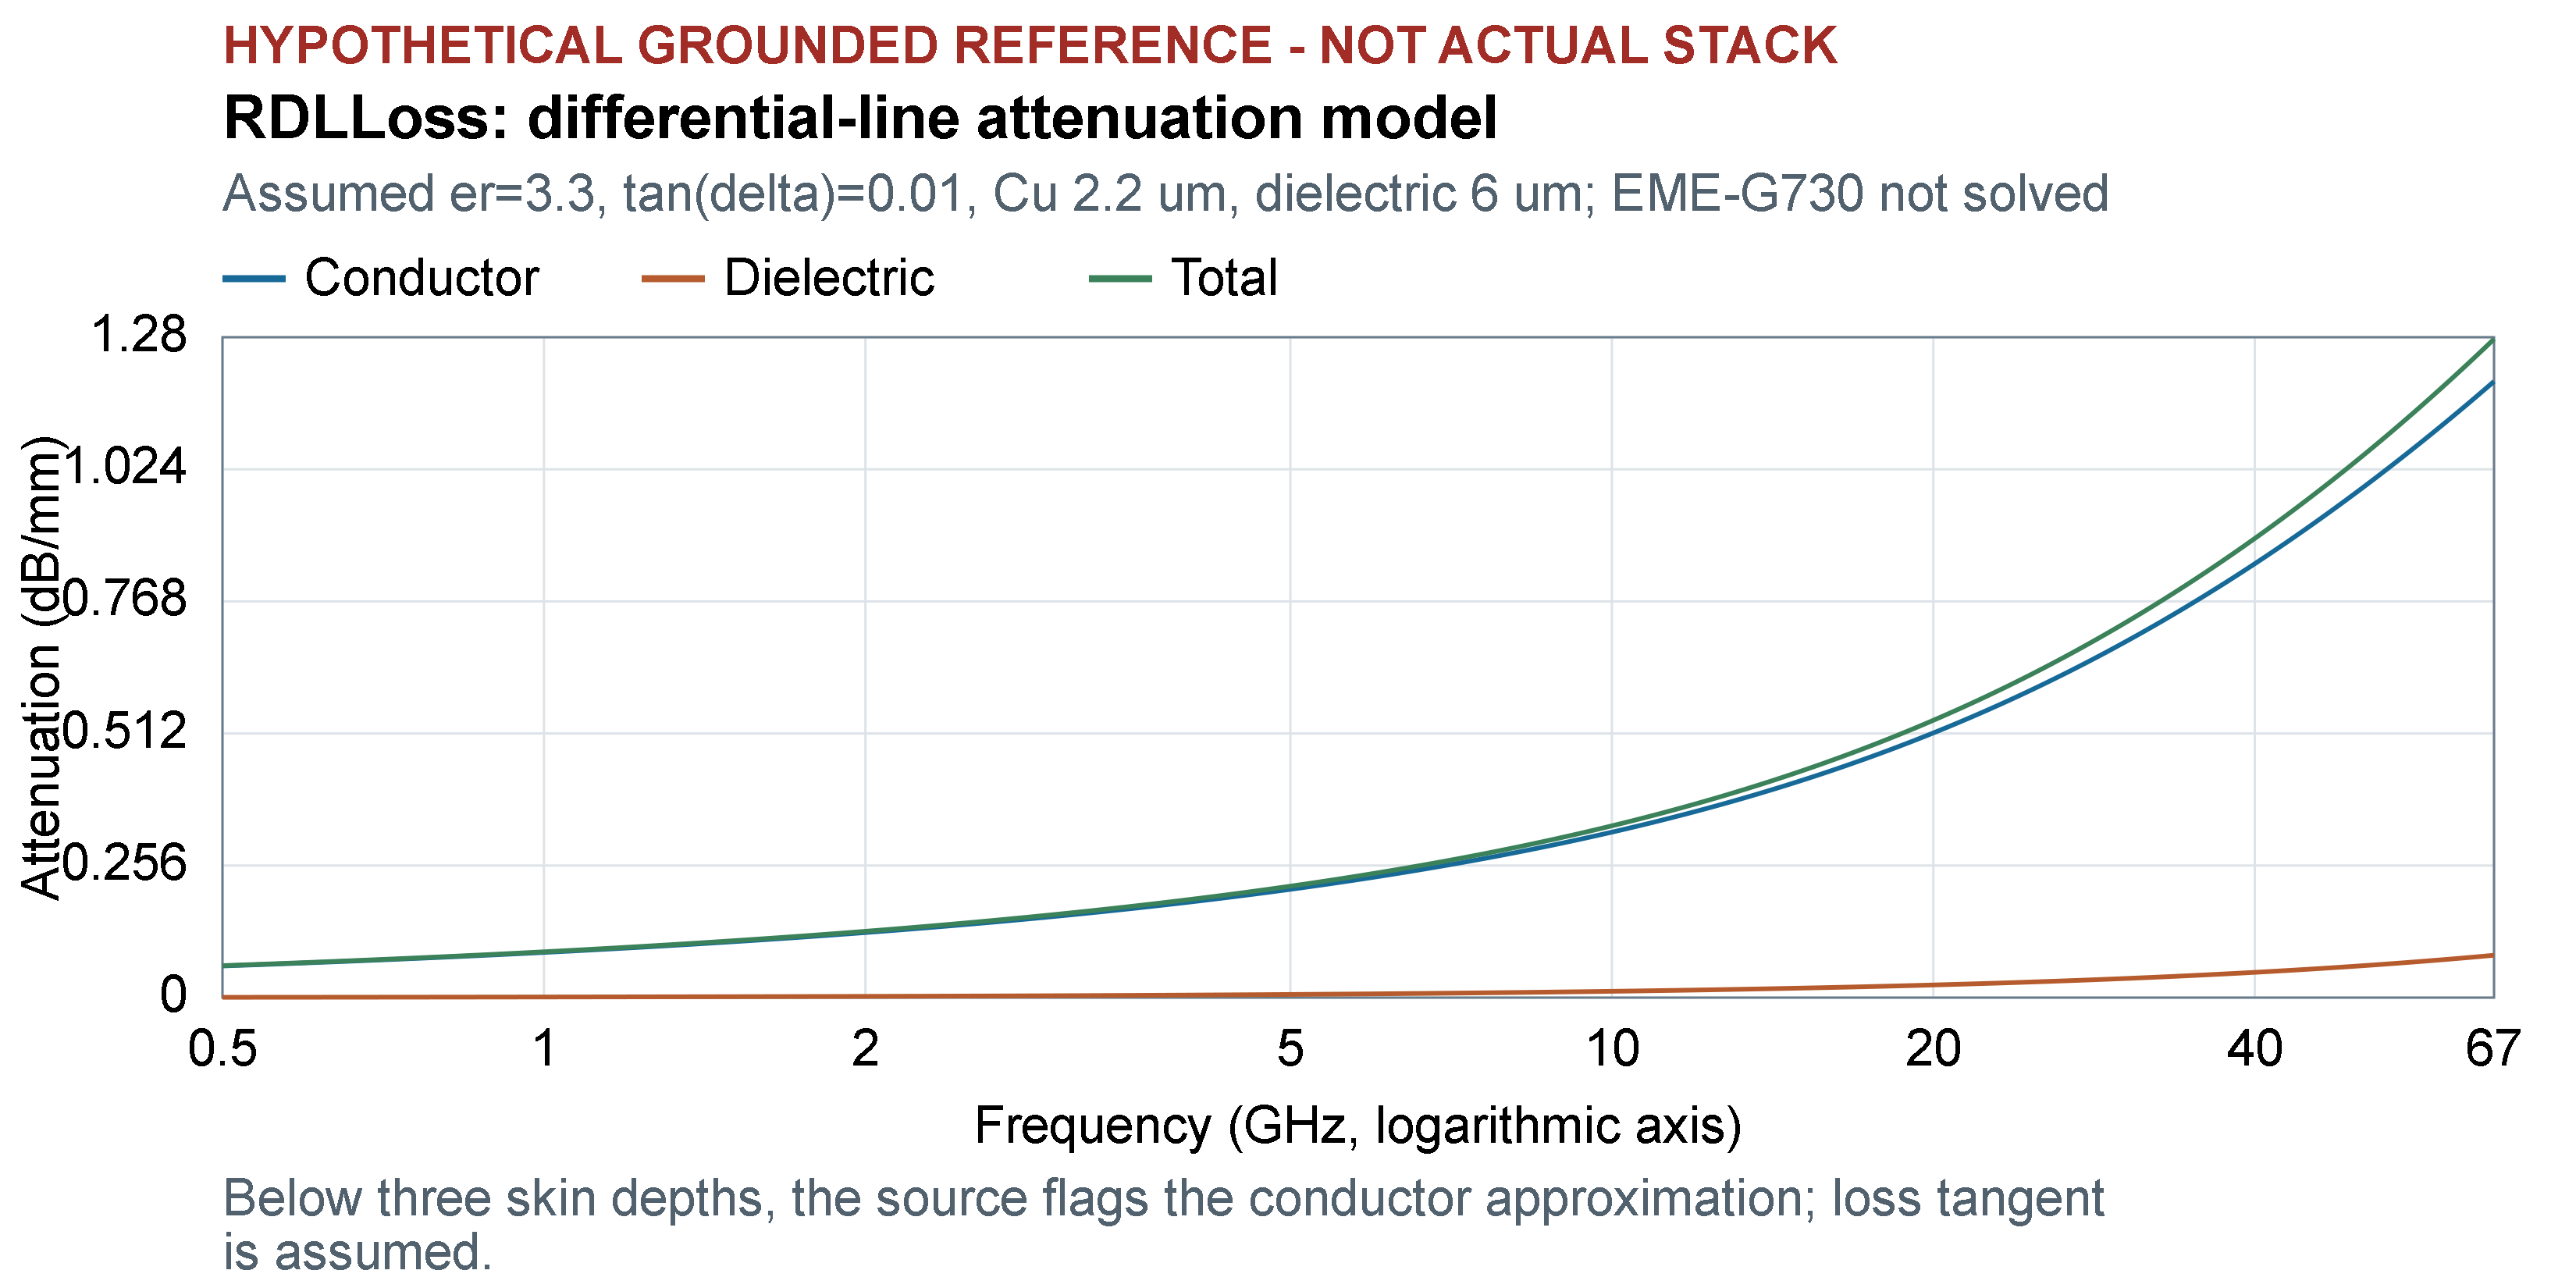
\includegraphics[width=.97\linewidth,height=.34\textheight,keepaspectratio]{assets/rdlloss-response.png}\end{center}
The gallery stores all seven response plots under a separate, initially collapsed reference section. Raw results, assumptions, source-line provenance and cross-check results are in \texttt{rf-results.json} and \texttt{rf-results.csv}. No actual-stack S-parameter file is generated.
\newpage
\pageTitle{Files, verification and next design steps}{Reproduce the previews and PDF without changing the BASIC listings}
\subhead{Delivered files}
\par\noindent\begin{tabular}{@{}p{.44\linewidth}p{.51\linewidth}@{}}\toprule
\texttt{handbasic-previews/index.html} & Preview gallery, with RF artwork, utility text and reference-plot sections.\\
\texttt{handbasic-preview-profile.json} & User stack and probes; explicit reference assumptions and model applicability.\\
\texttt{handbasic-previews/*.svg / *.png} & Editable vector artwork and viewing images.\\
\texttt{*-commands.json / *manifest.json} & Source commands, source/profile hashes, calculation entry points and limits.\\
\texttt{reports/build.ps1} & Regenerate previews, data, gallery and report with pdfLaTeX.\\
\texttt{reports/handbasic-ltc25000-eme-g730.tex} & Editable report source.\\
\texttt{reports/report\_math.mjs} & Equations, worked values and expected-data text; its self-checks fail the build if a relation disagrees with \texttt{rf-results.json}.\\
\texttt{gds/gds\_*.bas, gds/*.GDS} & Eight cbmbasic scripts and the generated GDSII unit cells with ground plane.\\
\texttt{gds/verify\_gds.mjs, gds/run\_gds.ps1} & Stream, geometry and connectivity checks; regenerate all cells.\\\bottomrule
\end{tabular}\par
Run \texttt{powershell -File reports/build.ps1} from the project folder. Node.js, ImageMagick and pdfLaTeX are required. The build checks that all RF manifests use the same profile and unchanged BASIC sources; mathematical text previews are literal extraction. Mobile app behavior, probe-body fit, fabricated dimensions and physical RF performance are not validated by this build.
\subhead{Scope of the program inventory}
All ten parent-folder BASIC programs are represented. The C64-only \texttt{RING67.PRG} is a separate synthetic ideal two-port model, not an additional Hand BASIC program; it is not a solver for this physical stack and is not presented as one.
\subhead{Before assigning fabrication dimensions or RF predictions}
Obtain the complex permittivity of both exact cured material grades over 0.5--67 GHz, together with copper conductivity/roughness and the support/chuck boundary. Define connected top-ground regions, CPW slots, optional bridges, the RFLEAK second metal layer and VIAMATCH return geometry. Then solve the finite-thickness multilayer CPW structures and launches, synthesize the nominal 50 ohm geometry, and check calibration on matching standards. Preserve the existing cardinal port counts and assignments during that redesign.
\subhead{Sources}
{\small
[1] MPI Corporation, \href{https://www.mpi-corporation.com/wp-content/uploads/ASTPDF/MPI-Probe-Selection-Guide.pdf}{Probe Selection Guide}, T67, p.6: 67 GHz family and available GSG pitches. Rating is a probe specification, not a guarantee for the DUT or the complete measurement system.\par
[2] EV Group / FUJIFILM, \href{https://www.swtest.org/swtw_library/2024proc/pdf/W06_03_VARGA_SWTest-2024.pdf}{SWTest 2024 digital-lithography process study}. Identifies LTC 25000 in process trials; it is not broadband dielectric characterization.\par
[3] Sumitomo Bakelite, \href{https://www.sumibe.co.jp/product/it-materials/epoxy/sumikon-eme/}{SUMIKON EME semiconductor encapsulants}. G730 Ver. GR and G314 are separate entries. Exact user grade suffix is unconfirmed.\par
[4] Qucs technical documentation, \href{https://qucs.github.io/tech/node86.html}{Coplanar waveguides}. Topology, finite-substrate and conductor-thickness considerations.\par
[5] Qucs technical documentation, \href{https://qucs.github.io/tech/node75.html}{Single microstrip line}. Source model family and thickness corrections.\par
}
\end{document}
